\chapter{Simulations of Cross-Beam Energy Transfer for Magnetised Direct-Drive}

This chapter describes a set of simulations which were conducted to understand the role of \ac{CBET} in magnetised, direct-drive implosions.
Magnetised \ac{ICF} is a promising route to achieving higher target gains, due to the reduction of hotspot thermal energy loss at stagnation and additional confinement of the alpha particles responsible for burn propagation.
For direct-drive implosions, magnetisation can significantly alter the coronal plasma conditions, due to the anisotropisation of thermal transport.
The \ac{IAW} dispersion relation, which mediates \ac{CBET} interactions, depends upon the background plasma and therefore significantly altered temperature and density profiles could alter the action of \ac{CBET}.
Before the development of \textsc{Solas}, no direct-drive suitable \ac{CBET} model existed, which was integrated into a \ac{Rad-MHD} code.
Therefore, the \textsc{Chimera}-\textsc{Solas} framework has enabled the effect of magnetisation on \ac{CBET} to be studied for a direct-drive implosion.

The chapter begins with a review of experimental and computational work on magnetised \ac{ICF}, with a particular focus on magnetised direct-drive.
Work presented in this chapter focuses on the study of `exploding-pusher' experiments.
These are very different implosions to the typical central hotspot ignition designs, presented in previous chapters, so a short summary of exploding-pushers is also provided.
1-D and 2-D simulation results are presented of unmagnetised exploding-pushers, both with and without the effect of \ac{CBET}, which demonstrate that \ac{CBET} does significantly affect these implosions.
This is followed by an investigation of how various extended-\ac{MHD} terms alter the implosion, including the Nernst effect, the Lorentz force and resistive diffusion of the magnetic field.
Results are given of how magnetisation affects the \ac{CBET} interaction and ultimately how it changes the stagnation shape of the target.
The results demonstrate that redistribution of deposited power due to \ac{CBET}, reduced the amplitude of the stagnation asymmetry, which originated from the polar beam configuration used.
However, the reduction of asymmetry was consistent for different initial seed magnetic field values, and therefore \ac{CBET} was not observed to be sufficiently strongly affected by magnetisation, to lead to observable signatures in experimental measurements.
The chapter concludes with a summary of the work conducted, and suggestions of additional experimental configurations, which may leave a more significant signature of magnetisation altering \ac{CBET}.

\newpage

%###############################################################################################################################
%###############################################################################################################################
%###############################################################################################################################
\section{Magnetised Inertial Confinement Fusion and Exploding-Pushers}%
\label{sec:Res2_MagICF}

This chapter begins with a review of published studies of relevance to the work conducted in this chapter.
Firstly, a short review of magnetised-\ac{ICF} is presented, which reviews both the key concepts, existing studies and potential challenges of the design.
Both work on direct- and indirect-drive is summarised, alongside recent theoretical progress on understanding how magnetisation can effect \ac{LPIs}.
The exploding-pusher concept is then briefly summarised to aid understanding of the implosion physics, which is markedly different to conventional hotspot \ac{ICF}.

%################################################################################
%################################################################################
\subsection{Potential Benefits of Target Magnetisation}%
\label{sec:Res2_magbenefits}

\begin{figure}[t!]
    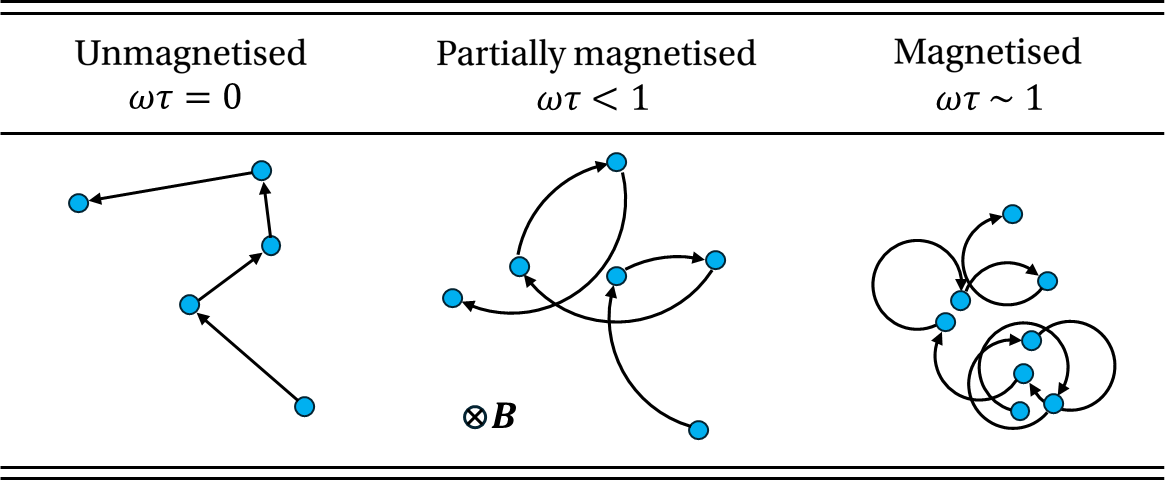
\includegraphics[width=0.75\linewidth]{Results2/Images/wt_collisions.png}
    \centering
    \caption{Cartoon to illustrate the effect of magnetisation on collisions, and therefore transport, of a test positive charge.
    Particle locations after collision are represented as blue circles and the path taken by the particle is shown by the black arrows.
    As the Hall parameter of the particle increases, diffusion is increasingly limited, and therefore collision transport is reduced.}%
    \label{fig:Res2_omegatau}
\end{figure}

Magnetisation of an \ac{ICF} target has long been thought of as a potential aid to ignition~\cite{lindemuth_parameter_1983,jones_physics_1986}.
It is still a relevant field of study in the context of regular ignition events on the \ac{NIF}, because by relaxing the ignition threshold, magnetisation could make larger targets feasible at an equivalent laser energy, and therefore lead to higher gains than unmagnetised implosions.
For a central hotspot ignition targets, ignition occurs when the heat source of alpha energy deposition balances the thermal and radiative losses in the hotspot.
Thermal conduction is suppressed perpendicular to magnetic field lines, therefore a magnetic field can reduce thermal losses and aid the power balance required for ignition.
Fig.~\ref{fig:Res2_omegatau} demonstrates the effect of increasing magnetisation on a unit positive test charge.
By constraining charged particles to orbit field lines, collisional transport terms, such as thermal conduction, are reduced perpendicular to the field direction.
Fits of transport coefficients to Fokker-Planck simulations, demonstrate that in a Hydrogen plasma, thermal conductivity perpendicular to field lines, $\kappa_{\perp}$, is reduced to $\sim$30\% of the parallel value, $\kappa_{\parallel}$, at Hall parameter, $\omega\tau=1$, and $\sim$1\% at $\omega\tau=10$~\cite{epperlein_plasma_1986}.
Thus, for Hall parameters, $\omega\tau\gtrsim 10$, thermal conduction losses are almost negligible in the direction perpendicular to field lines.

Using an order of magnitude estimate for a below ignition threshold hotspot, $T_e\sim 2.5\ \text{keV}$ and $\rho\sim50\ \text{g cm}^{-3}$, a field strength $|\vec{B}|\sim 2.5\ \text{kT}$ is required to obtain $\omega\tau\sim1$~\cite{oneill_modelling_2023}.
This field strength cannot be produced directly, but it is possible to produce a smaller field which, assuming frozen in magnetic field and a spherical compression, is amplified by the square of the convergence,
\begin{equation}
    \label{eq:Res2_flux_compression}
    |\vec{B_1}|=|\vec{B_0}| \left(\frac{R_0}{R_1}\right)^2,
\end{equation}
where $|\vec{B_0}|$ and $|\vec{B_1}|$ are initial and final magnetic fields, respectively and $R_0$ and $R_1$ are initial and final radii, respectively.
Laboratory magnetic fields can be produced from pulsed power coils with field strength $|\vec{B}|\sim\mathcal{O}(50)\ \text{T}$~\cite{fiksel_note_2015}, so even moderate convergence-ratio targets ($R_0/R_1\sim10$) are able to produce strongly magnetised core plasma.

\begin{figure}[t!]
    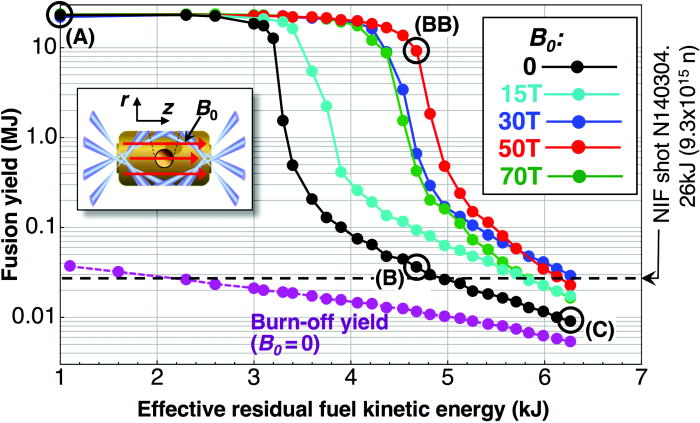
\includegraphics[width=0.75\linewidth]{Results2/Images/magicf_perkins.jpeg}
    \centering
    \caption{Simulated fusion yields versus effective residual fuel kinetic energy under imposed low-mode radiation flux perturbations for imposed fields in the range $B_0=0\rightarrow70\ \text{T}$.
    The plot demonstrates, that with increasing departure from ideal compression (moving to the right on the $x$ axis), magnetisation can enable the onset of the ignition.
    Reused with permission from Ref.~\cite{perkins_potential_2017}.}%
    \label{fig:Res2_perkins_magicf}
\end{figure}

Fig.~\ref{fig:Res2_perkins_magicf} plots results of magnetised indirect-drive simulations, for a target on the threshold of ignition~\cite{perkins_potential_2017}.
Increasing magnitude of radiation perturbation were applied to the drive (moving to the right on the $x$-axis), which prevent the target from achieving ignition, which is visible as the steep increase in yield, below some threshold level of perturbation.
The results demonstrate that when an initial magnetic field was applied to the target, it more robustly ignited with increasing field strength, due to reduced conduction losses.
This simulation work, prior to the achievement of ignition on the \ac{NIF}~\cite{zylstra_burning_2022}, motivated the development of a magnetised \ac{ICF} campaign at \ac{LLNL}~\cite{moody_magnetized_2022}.

The \textsc{Chimera} code has been used to study a wide array of physics relevant to magnetised \ac{ICF}.
Simulation work has been conducted, which has shown that magnetisation can alter instability growth of magnetised laser fusion implosions.
While in the deceleration phase, magnetic tension can reduce low-mode perturbation growth~\cite{walsh_perturbation_2019}, magnetisation of directly-driven targets inhibits heatflow in the plasma corona and thus limits thermal stabilisation of short wavelength modes from laser imprint~\cite{walsh_magnetized_2020}.
Recent work has also demonstrated that magnetisation of high-yield, indirect-drive targets must be carefully optimised, in order to avoid significant degradation to the implosion shape, due to anisotropic thermal conduction and inhibition of burn propagation from $\alpha$ magnetisation~\cite{oneill_modelling_2023}.

%################################################################################
%################################################################################
\subsection{Experimental Studies of Magnetised-ICF}%
\label{sec:Res2_magicf_prevwork}

\begin{figure}[t!]
    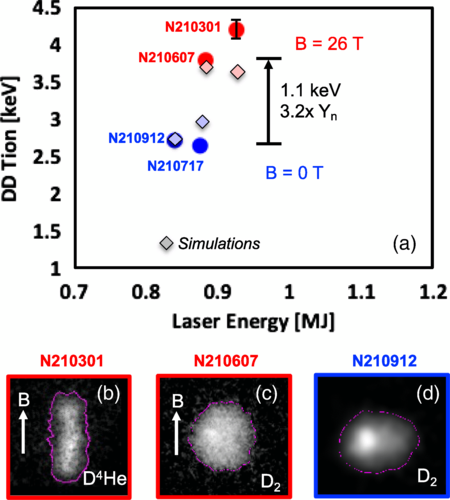
\includegraphics[width=0.5\linewidth]{Results2/Images/magnif_yield_inc.png}
    \centering
    \caption{a) A 1.1 keV $T_i$ increase was achieved by adding a 26 T $B_0$ field to a D${}_{2}$ gas capsule implosion on the \ac{NIF}.
    Also shown in the plot are the simulation results.
    b)$\rightarrow$d) Equatorial shapes of the implosions.
    Reused with permission from Ref.~\cite{moody_increased_2022}.}%
    \label{fig:Res2_moody_magnif}
\end{figure}

Indirect-drive experiments have been conducted on the \ac{NIF} to demonstrate the efficacy of magnetised targets, in reducing thermal conduction losses in the hotspot.
Non-cryogenic, deuterium filled capsules were deployed with initial field strengths up to $26\ \text{T}$~\cite{moody_increased_2022}.
Results from this experimental campaign are show in Fig.~\ref{fig:Res2_moody_magnif}.a.
The magnetised targets demonstrated significantly enhanced ion temperatures and neutron yields and work is underway to explore non-uniform field configurations to further enhance the benefits of magnetisation~\cite{walsh_application_2023}.
Fig.~\ref{fig:Res2_moody_magnif}.b,~\ref{fig:Res2_moody_magnif}.c and ~\ref{fig:Res2_moody_magnif}.d plot x-ray images at stagnation of different experiments, showing that a shape-tuning process had to be conducted in order to optimise the sphericity of the target, due to the field leading to anisotropic thermal conduction.

\begin{figure}[t!]
    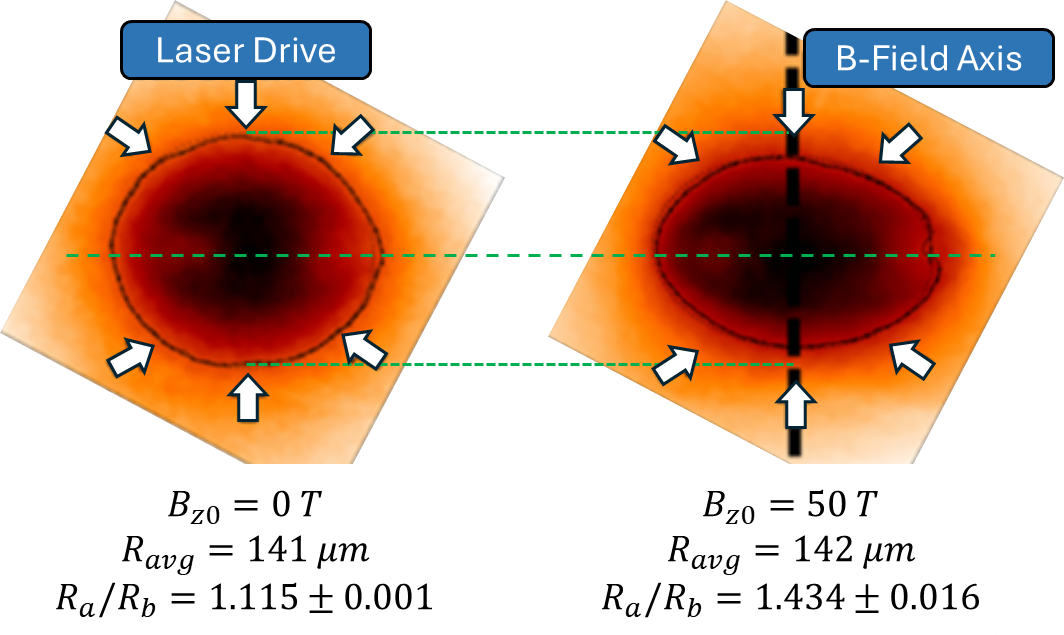
\includegraphics[width=0.6\linewidth]{Results2/Images/MagP2_Bose.png}
    \centering
    \caption{X-ray self emission images of (left) an unmagnetised and (right) a magnetised implosion.
    The average radius of the marked contour (corresponding to 40\% of peak intensity), and the oblateness parameter $R_a/R_b$ (ratio of major-to-minor axis) are listed below each image.
    The polar laser-drive is indicated by the white arrows, and the axis of the initial magnetic field by the black dashed line on the right.
    Applying an initial magnetic field demonstrated increased oblateness of the implosion.
    Adapted with permission from Ref.~\cite{bose_effect_2022}.}%
    \label{fig:Res2_Bose_magp2}
\end{figure}

Magnetisation of direct-drive targets has been investigated by experiments on the \textsc{Omega} laser facility for a number of years.
Initial \textsc{Omega} experiments focussed on verification of magnetic flux compression, by applying an initial seed field along the axis of a cylinder that was imploded via laser irradiation~\cite{gotchev_laser-driven_2009}.
The magnetised implosions validated predictions of flux compression and demonstrated enhanced neutron yields and core ion temperatures over unmagnetised implosions.
Spherical targets were subsequently fielded, which also resulted in increased stagnation temperatures and yield compared to unmagnetised targets~\cite{chang_fusion_2011,hohenberger_inertial_2012}.
No noticeable degradation to the implosion shape or performance was observed in these experiments, which was assumed to be due to the high ratio of plasma pressure to magnetic pressure, $\beta\gg 1$.

The most recent experimental, magnetised direct-drive work has focussed on exploring higher initial seed field values ($|\vec{B}_0|\sim50\ \text{T}$ compared to $|\vec{B}_0|\sim8\ \text{T}$), to understand the saturation of performance with increasing field.
A shock-driven, exploding-pusher target configuration was used for these experiments, in order to create high ion temperatures and thus create a platform to study magnetised ions.
Exploding-pushers are significantly different implosions compared to hotspot ignition targets discussed in previous chapters and shall be described in detail in Sec.~\ref{sec:Res2_expl}.
Creating these strong, $50\ \text{T}$ fields at the target necessitated reducing the radius of the equatorial field coil compared to previous experiments.
Therefore, a 40-beam configuration had to be used, without the 20 equatorial beams, leading to a pole-heavy laser drive.
The high fields of these implosions led to strongly magnetised coronal electrons, $\omega_e\tau_e\sim50$, resulting in strongly anisotropic thermal conduction $\kappa_{\perp,e}/\kappa_{\parallel,e}\sim10^{-4}$.
This is compared to previous experiments which produced $\omega_e\tau_e\sim1$ and therefore $\kappa_{\perp,e}/\kappa_{\parallel,e}\sim1/3$.
For direct-drive on \textsc{Omega}, laser deposition is transported to the ablation surface by electron thermal conduction, thus large electron Hall parameters led to an effective anisotropisation of the implosion drive.

Fig.~\ref{fig:Res2_Bose_magp2} shows x-ray self-emission images of an unmagnetised (left) and magnetised (right) target with an initial $|\vec{B}_0|=50\ \text{T}$ seed field.
The strongly magnetised coronal electrons led to decreased drive $\perp\hat{\vec{B_0}}$, markedly increasing the oblateness of the diagnostic image compared to the unmagnetised target.
An ion magnetisation of $\omega_i\tau_i\sim7$ was also reported.
Previous \ac{Rad-MHD} modelling of these experiments, using the \textsc{Chimera} code, did not include the effects of \ac{CBET}.
The development of \textsc{Solas}, and particularly the \ac{CBET} model, motivated further computational study of these experiments, to explore whether \ac{CBET} played a significant role in dictating the shape of these implosions.
This is because \ac{CBET} is known to markedly compensate global, $\ell=1$ asymmetries~\cite{anderson_effect_2020,colaitis_inverse_2021}, therefore the anisotropy introduced from magnetisation could affect the action of \ac{CBET}.

%################################################################################
%################################################################################
\subsection{Magnetised Laser-Plasma Instabilities}%
\label{sec:Res2_maglpis}

Sec.~\ref{sec:Res2_mag_on_CBET}, aims to understand how magnetisation of a direct-drive implosion anisotropically changes the hydrodynamics, and how these altered coronal plasma conditions modify the calculated \ac{CBET} gains, discussed in Sec.~\ref{sec:SOLAS_ray_power_change}.
For example, magnetisation restricts thermal conduction and therefore enhances coronal electron temperatures along the initial field axis.
Approximately, the fluid \ac{CBET} gain, $\gamma_{ij}\propto T_e^{-1}$, therefore anisotropic changes to $T_e$ could result in reduced \ac{CBET} gains around the target and therefore change \ac{CBET} scattering compared to implosions without an applied field.
This modification to \ac{CBET} via the altered hydrodynamic profiles is called the \textit{indirect} effect of magnetisation on \ac{LPIs}.

Magnetisation can, however, also \textit{directly} modify scattering from \ac{LPIs}, in a number of ways.
For \ac{ICF} conditions, when the field strength is sufficiently high, electron cyclotron motion can become comparable to plasma wave frequencies, and therefore alter the dispersion relation of the mediating plasma wave in \ac{LPIs}.
In underdense, \ac{ICF} relevant plasma ($n_e \sim 10^{20}\ \text{cm}^{-3}$ and $T\sim2\ \text{keV}$), the \ac{IAW}, which mediates \ac{SBS} and \ac{CBET}, is significantly modified when $|\vec{B}|\sim100\ \text{T}$ and the \ac{EPW}, which mediates \ac{SRS} and \ac{TPD}, when $|\vec{B}|\sim1000\ \text{T}$~\cite{shi_benchmarking_2023}.
Additionally, the (predominantly collisionless) damping of plasma waves can also be modified, because cyclotron motion of particles can affect their trapping in plasma waves~\cite{shi_benchmarking_2023}.
Significant theoretical progress has been made in this field in recent years by Shi \text{et al.}, who derived analytic formulae for 3 wave coupling in the presence of a magnetic field \cite{shi_three-wave_2017,shi_laser-plasma_2018}.
This was a challenging problem, due to the lack of simple geometries for the interaction, when a field is applied to a plasma with an arbitrary direction.

The simulation results here neglect this direct affect of magnetisation on \ac{CBET}, partially because the theory is not yet deemed to be significantly mature, to implement within a reduced, ray-based model.
Additionally, coronal magnetic field strengths of $|\vec{B}|\lesssim50\ \text{T}$ were observed in the underdense coronal plasma so significant modifications to the \ac{IAW} dispersion relation were not expected.
It is noted, however, that altered damping of the waves from magnetisation may affect the results, but the focus of the study was predominantly to explore how magnetisation might indirectly affect \ac{CBET}.

%################################################################################
%################################################################################
\subsection{The Exploding-Pusher Configuration}%
\label{sec:Res2_expl}

Exploding-pushers are considered to be a highly reproducible platform, robust to instabilities and capable of producing large neutron yields.
Although historically it had a slightly different meaning~\cite{craxton_direct-drive_2015}, the term `exploding-pusher' is now, typically used for low convergence, thin-shell targets~\cite{ellison_development_2018}.
When irradiated with significant intensity, frequency-tripled laser light\footnote{When frequency-tripled light is not used, suprathermal electrons, rather than ablation, is the dominant driver of the strong shock~\cite{yeamans_high_2021}.}, the thin shell rapidly heats and then explosively ablates, driving a strong shock radially inward, ahead of the majority of in-falling ablated material.
This shock strongly heats the ions as it propagates through gas-fill to large, fusion relevant temperatures.
After rebounding from the axis, the shock recompresses the infalling exploded shell material, resulting in sufficient density for a significant number of fusion reactions.

Directly-driven exploding-pusher targets have the largest direct-drive fusion yields recorded on the \ac{NIF}, resulting in $E_{\text{fusion}}\sim 30\ \text{kJ}$ \cite{yeamans_high_2021}.
However, they are not suitable for high gain designs, as the low areal densities of the target are not sufficient to confine $\alpha$ particles and thus enable burn propagation.
A variety of interesting physics may be studied using the platform due to the significant ion temperatures that can be achieved, such as equilibration between electrons and ions~\cite{benedict_molecular_2012} and kinetic effects in the ion population~\cite{mannion_evidence_2023}.
The strong shock is also highly kinetic, and thus accurate comparison to experimentally measurable variables, such as yields and ion temperatures, is expected to be difficult for \ac{Rad-Hydro} codes which neglect kinetic effects~\cite{larroche_ion-kinetic_2016}.
However, much of the key dynamics and results can be studied more qualitatively.

%###############################################################################################################################
%###############################################################################################################################
%###############################################################################################################################
\section{Cross-Beam Energy Transfer in Unmagnetised Exploding-Pushers}%
\label{sec:Res2_CBET_expl}

This section presents simulation results, which demonstrate the effect of \ac{CBET} in exploding-pushers on \textsc{Omega}.
Both 1-D and 2-D \textsc{Chimera}-\textsc{Solas} simulations of 40-beam, pole-heavy drive, exploding-pusher experiments are presented, with a focus on how \ac{CBET} acts to change the implosion.
The 1-D results demonstrate that \ac{CBET} significantly reduced the coupled laser energy to the implosion from $81.1\%$ to $69.7\%$.
Simulations conducted in 2-D, with a full 3-D raytrace and \ac{CBET} model, clearly demonstrated that the polar drive configuration led to an oblate implosion. 

%################################################################################
%################################################################################
\subsection{Simulation Configuration}%
\label{sec:Res2_simconfig}

\begin{figure}[t!]
    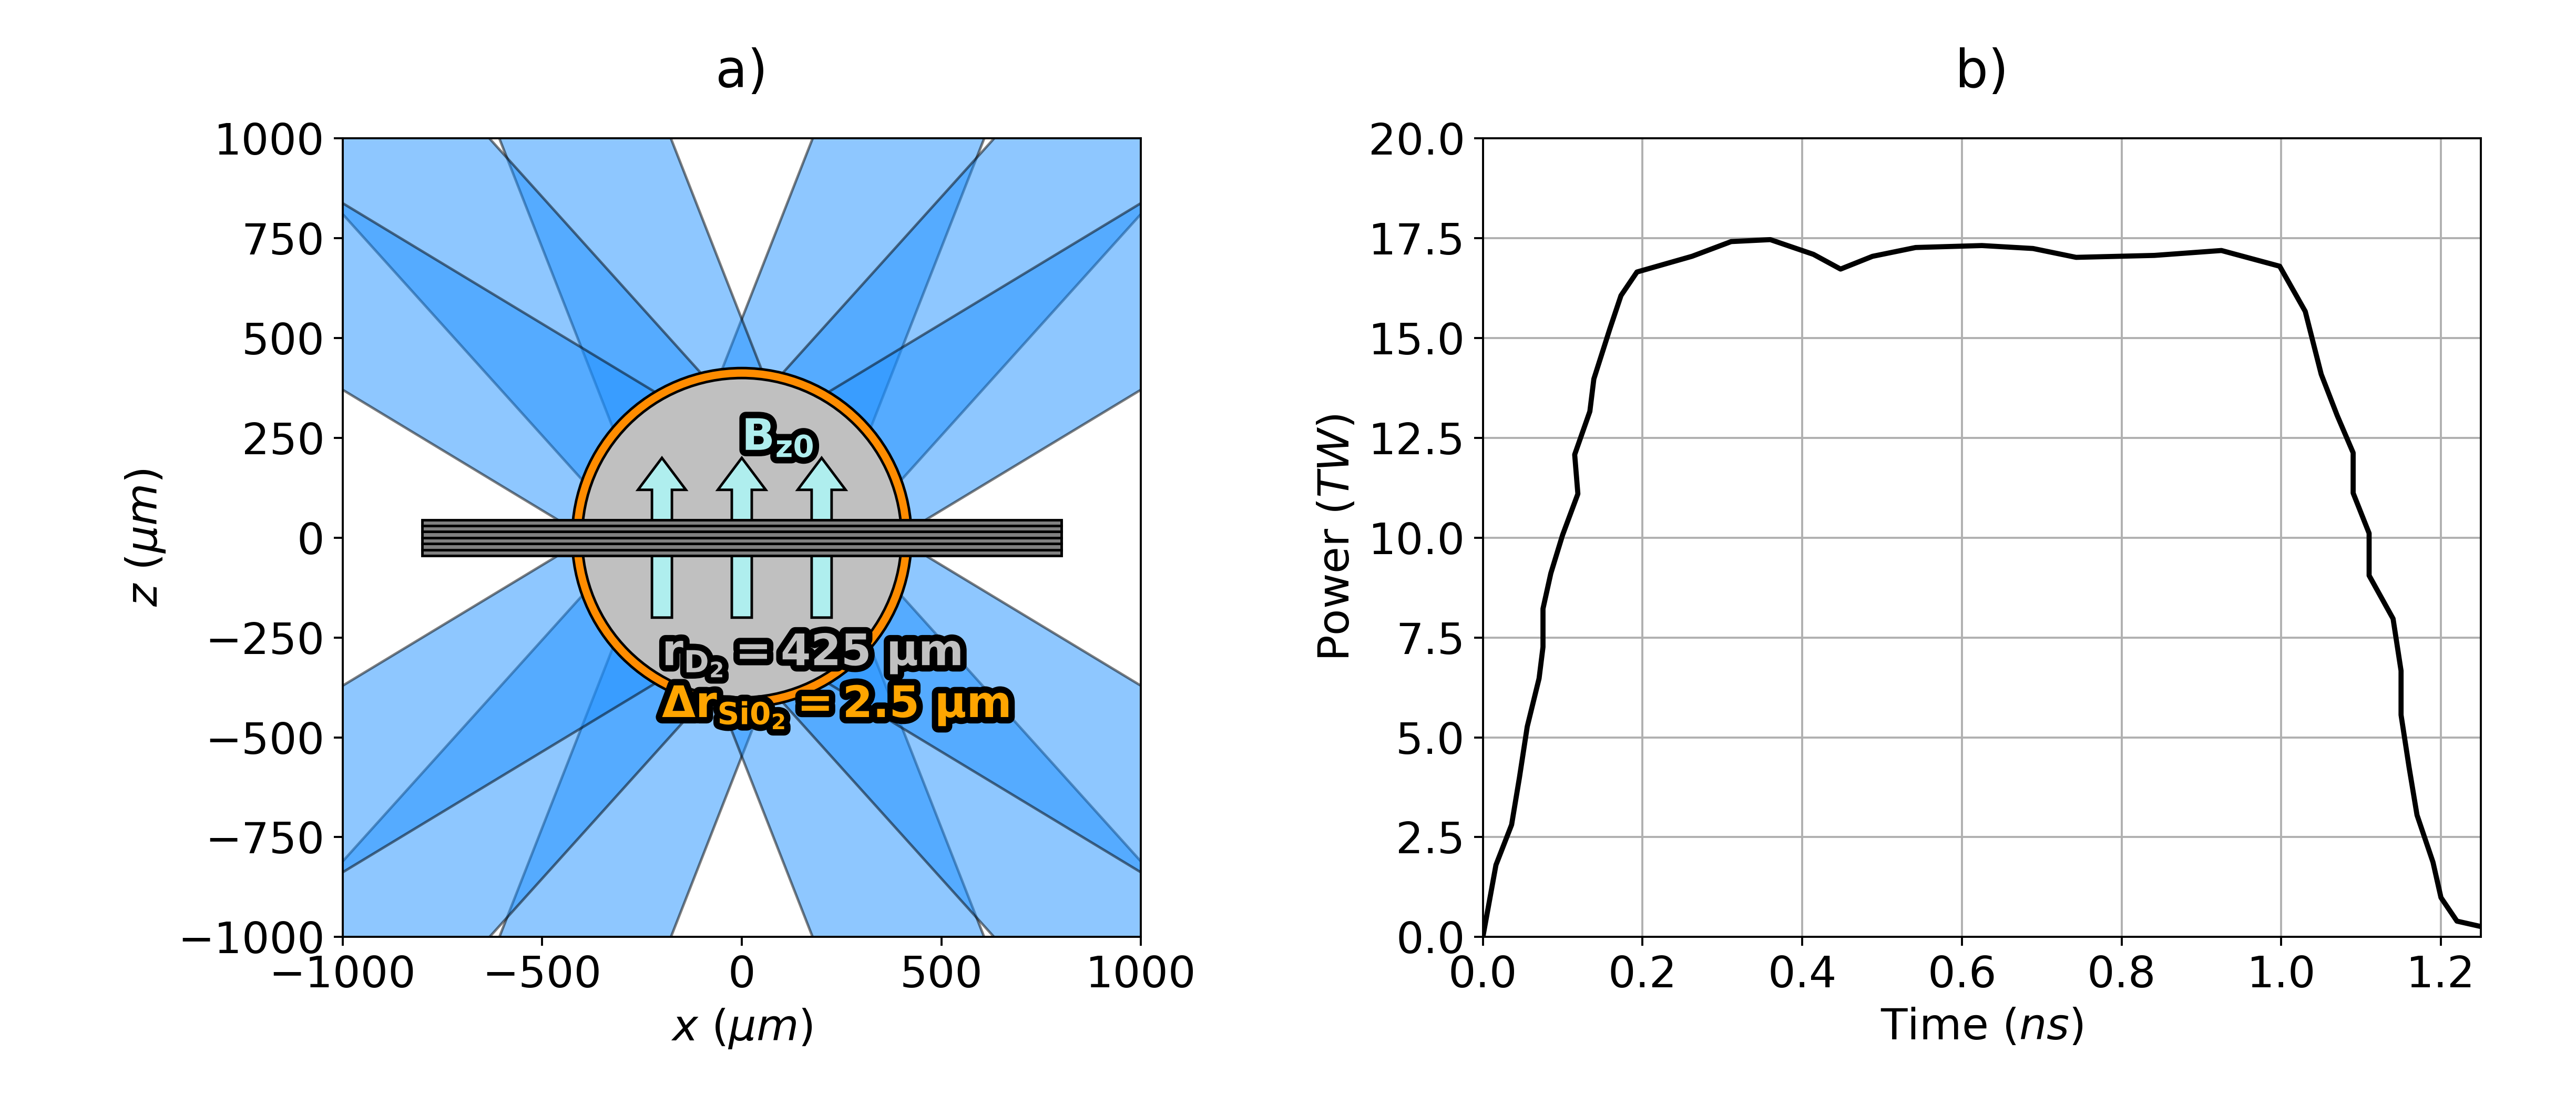
\includegraphics[width=\linewidth]{Results2/Images/magpdd_diagram_pulse.png}
    \centering
    \caption{The initial conditions used for all simulations presented in this chapter.
    Panel a) plots the D${}_{2}$ filled, glass shell capsule and direction of the initial magnetic field.
    An example field coil (illustrative and not included in simulations) is also shown, the presence of which necessitated the polar laser drive in experiments.
    Panel b) plots the laser pulse shape used, which had a total of $17.7\ \text{kJ}$ laser energy.}%
    \label{fig:Res2_simconfig}
\end{figure}

The simulations conducted for this chapter aimed to study experimental configurations similar to the results from Bose \textit{et al.}, discussed in Sec.~\ref{sec:Res2_magicf_prevwork}~\cite{bose_effect_2022}.
Experimental data from these magnetised exploding-pushers, demonstrated a clear amplification of the mode-2 due to magnetisation, which could have affected \ac{CBET} scattering.
The beam configuration, capsule initial conditions and pulse shape used for all simulations in this chapter are shown in Fig.~\ref{fig:Res2_simconfig}.
The exact pulse shape and target specifications were from a set of follow-up experiments to Bose \textit{et al.} and were provided by C. W. Chang and J. Frenje from \ac{MIT}~\cite{chang_notitle_2023}.
40 beams from the \textsc{Omega} laser, delivered a total of $17.7\ \text{kJ}$ laser energy to a $2.5\ \mu\text{m}$ thick, glass ($\text{SiO}_2$)\footnote{By ion number density, the material comprised $1/3$ $\text{Si}$ and $2/3$ $\text{O}$.} capsule, filled with room temperature and pressure $\text{D}_2$.
All experiments removed the 20 equatorial beams from the drive, because the presence of the small radius field coil in experiments precluded them.
Magnetic fields of strength $B_{z0}=0$, $25$ and $50\ \text{T}$ were applied along the z-axis of the configuration for different simulations.

An explicit $P_{1/3}$ radiation transport algorithm was used for all simulations, using tabulated opacities and emissivities from the \textsc{SpK} code~\cite{crilly_spk_2023}.
A tabulated \texttt{Sesame} equation of state was employed for each material~\cite{mchardy_introduction_2018}.
The \textsc{Chimera} extended-\ac{MHD} package was used, which included resistive diffusion of the magnetic field, Lorentz force of the magnetic field on the hydrodynamics, Nernst advection of the field down temperature gradients and anisotropic thermal conduction~\cite{walsh_extended-magnetohydrodynamics_2020}.
Thermal conduction was solved using a Super-time-stepping, semi-implicit algorithm~\cite{vaidya_scalable_2017}, with flux-limited, Spitzer conductivities~\cite{spitzer_transport_1953}.
An electron flux limiter of $f_{\text{lim},e} = 0.15$ was set for all simulations.
Exploding-pushers exhibit high coronal temperatures due to the high-$Z$ ablator and large temperatures for the strong imploding shock, therefore simulation yields and bangtimes are highly sensitive to thermal conduction and the choice of flux limiter.
Although not the focus of this work, if attempting to match simulation result to experimental yields, reducing the flux limiter value would strongly inhibit the drive and therefore reduce simulation bangtimes.
The flux limiter would therefore be the primary parameter to vary, in order to obtain better match the integrated results to experimental values.
In order to improve the speed of the thermal conduction algorithm, which severely limited the stable simulation timesteps on vacuum-plasma interfaces, an artificial material was placed outside the capsule, which had an enforced ionisation state of $Z=0$.
This had minimal impact on the implosion results, but significantly sped up simulation run-times.
The presence of the material did create large viscous heating of the ions as the coronal plasma expanded into it, which is visible in results throughout the chapter.
However, this viscously heated layer was well separated from the region of interest (near critical density) for the majority of the implosion, and therefore did not impact upon the results.

All simulations used a spherical-polar \textsc{Chimera} mesh, with a fixed radial resolution of $0.5\ \text{um}$, over the full $4\pi\ \text{str}$.
1-D simulations were run from beginning to end in spherical with $r\in[0,1400]\ \mu\text{m}$.
2-D calculations assumed azimuthal symmetry of the hydrodynamics and conducted an initial `drive-phase' in spherical coordinates, with $r\in[80,1400]\ \mu\text{m}$, where the central cutout region was removed to avoid taking small radiation transport timesteps due to the small cell faces close to the axis.
The 2-D drive-phase grid used 120 cells in the polar direction.
When the shock reached this cutout region, hydrodynamic variables were trilinearly interpolated onto a 2-D cylindrical ($r_{\text{cyl}},z$) mesh for the `stagnation-phase', with fixed resolution, $\Delta_{r,\text{cyl}}=\Delta_z=1\ \mu\text{m}$, and simulation bounds $r_{\text{cyl}}\in[0,1200]\ \mu\text{m}$ and $z\in[-1200,1200]\ \mu\text{m}$.
This grid contained no singularities, unlike a 2-D spherical grid without a cutout, and therefore excessively small radiation transport timesteps were not an issue.

All simulations used a 3-D laser ray-trace with a variety of \ac{CBET} treatments.
\ac{CBET} was fully included for some simulations and neglected for others.
Alternatively, partial-\ac{CBET} simulations were conducted to explore the effect that \ac{CBET} \textit{spatial redistribution} of deposited power had on implosions.
These simulations were conducted without the \ac{CBET} model, but were forced to deposit the same magnitude of power that was absorbed from the equivalent \ac{CBET} simulation.
Explicitly, a no-\ac{CBET} ray-trace was conducted, where the power of all rays was normalised to unity.
When this raytrace was complete, it read in the absorbed power from the (previously conducted) \ac{CBET} simulation at that time, and multiplied the (normalised) deposited power by this value.
This created a hydrodynamically similar implosion to the \ac{CBET} ray-trace, and via comparison of these two simulations, the impact of \ac{CBET} redistribution-of-deposition upon the hydrodynamics was studied.
Temporally-and-spatially integrated results from all simulations are presented in Tab.~\ref{tab:Res2_magexpl_results}, and are referred to when relevant throughout the chapter.

Several metrics have been included in the table, which are explicitly defined here.
The metrics are commonly used to compare implosions in \ac{ICF}, because, apart from the oblateness parameter in the last column, they can all be directly computed from experimental neutron spectra~\cite{frenje_nuclear_2020}.
As previously stated, bangtime is defined as the time of peak neutron production, which for this simulation, assumes only deuterium-deuterium reactions contribute,
\begin{equation}
    t_b = \text{argmax}_t \left( \int\ Y_{DD}(\vec{x},t)\ \text{d}V \right),
\end{equation}
where $Y_{DD}$ is the deuterium-deuterium neutron production rate, which is calculated across the \textsc{Chimera} computational grid at all locations and times throughout the simulation, using Bosch-Hale fits to the reactivity~\cite{bosch_improved_1992}.
The total neutron yield is the spatially and temporally integrated neutron production,
\begin{equation}
    Y_{n} = \int\int\ Y_{DD}(\vec{x},t)\ \text{d}V\text{d}t.
\end{equation}
The burn-width, $\Delta_b$ is the full width half maximum of the spatially integrated neutron production.
One interpretation of this diagnostic, for this very two-dimensional configuration, is that a highly oblate implosion will have less temporally and spatially localised convergence.
Therefore, neutron production for less symmetric implosions will likely happen over a longer timescale, because thermonuclear conditions are produced at different times in different locations.
The burn-averaged ion temperature, $\langle T_i \rangle$, is defined as the ion temperature, weighted by temporally and spatially resolved neutron production,
\begin{equation}
    \langle T_i \rangle = \frac{\int\int\ T_i(\vec{x},t) Y_{DD}(\vec{x},t)\ \text{d}V\text{d}t}{Y_{n}}.
\end{equation}
It is an integrated metric, which summarises the average temperature of the regions which are key in producing fusion-yield.
Finally, the oblateness parameter in the final column of the table, $(R_{\text{equator}}/R_{\text{pole}})|_{t=t_b}$, was obtained by fitting an ellipse (with axes orientated along $\hat{\vec{x}}$ and $\hat{\vec{z}}$), to the spherical radius of maximum density at bangtime.
The fitting procedure also returned asymmetric error bars, which are presented alongside the result.

%################################################################################
%################################################################################
\subsection{1-D Simulations}%
\label{sec:Res2_expl1D}

\bgroup%
\def\arraystretch{1.3}%  1 is the default, change whatever you need
% Please add the following required packages to your document preamble:
% \usepackage{multirow}
\begin{table}[]
    \centering
    \caption{Spatially and temporally integrated results from all Simulations. In the \ac{CBET} column, `$\sim$' indicates partial-\ac{CBET}, where \ac{CBET} reduced absorption magnitude, but \textit{not} spatial location, of deposition.}
    \begin{tabular}{cccccccccc}
        \hhline{==========}
        Run & Dim. & CBET   & Note      & \begin{tabular}[c]{@{}c@{}}$B_{z0}$\\ $(\mathrm{T})$\end{tabular} & \begin{tabular}[c]{@{}c@{}}$t_b$\\ $(\mathrm{ns})$\end{tabular} & \begin{tabular}[c]{@{}c@{}}$\langle T_i \rangle$\\ (keV)\end{tabular} & \begin{tabular}[c]{@{}c@{}}$Y_n$\\ $(\times10^{10})$\end{tabular} & \begin{tabular}[c]{@{}c@{}}$\Delta_b$\\ (ps)\end{tabular} & $\frac{R_{\text{equator}}}{R_{\text{pole}}}\bigg|_{t=t_b}$              \\ \hline
        1   & 1-D  & Off    & -         & 0                                                                 & 0.69                                                            & 14.66                                                                 & 11.62                                                            & 87                                                        & $1.00_{-0.00}^{+0.00}$ \\
        2   & 1-D  & On     & -         & 0                                                                 & 0.78                                                            & 12.37                                                                 & 10.57                                                            & 78                                                        & $1.00_{-0.00}^{+0.00}$ \\
        3   & 2-D  & Off    & -         & 0                                                                 & 0.71                                                            & 8.44                                                                  & 6.20                                                             & 148                                                       & $2.96_{-0.19}^{+0.20}$ \\
        4   & 2-D  & $\sim$ & -         & 0                                                                 & 0.75                                                            & 7.61                                                                  & 5.23                                                             & 153                                                       & $3.26_{-0.23}^{+0.25}$ \\
        5   & 2-D  & On     & -         & 0                                                                 & 0.75                                                            & 7.77                                                                  & 5.46                                                             & 148                                                       & $3.23_{-0.23}^{+0.25}$ \\
        6   & 2-D  & Off    & -         & 25                                                                & 0.74                                                            & 7.26                                                                  & 4.73                                                             & 130                                                       & $3.80_{-0.33}^{+0.41}$ \\
        7   & 2-D  & $\sim$ & -         & 25                                                                & 0.78                                                            & 6.58                                                                  & 4.14                                                             & 125                                                       & $4.55_{-0.43}^{+0.50}$ \\
        8   & 2-D  & On     & -         & 25                                                                & 0.78                                                            & 6.72                                                                  & 4.44                                                             & 123                                                       & $4.32_{-0.41}^{+0.47}$ \\
        9   & 2-D  & Off    & -         & 50                                                                & 0.73                                                            & 6.82                                                                  & 3.73                                                             & 134                                                       & $4.40_{-0.38}^{+0.43}$ \\
        10  & 2-D  & $\sim$ & -         & 50                                                                & 0.78                                                            & 6.30                                                                  & 3.30                                                             & 130                                                       & $4.92_{-0.48}^{+0.56}$ \\
        11  & 2-D  & On     & -         & 50                                                                & 0.78                                                            & 6.37                                                                  & 3.52                                                             & 129                                                       & $4.79_{-0.47}^{+0.55}$ \\
        12  & 2-D  & Off    & No Aniso. & 25                                                                & 0.81                                                            & 6.40                                                                  & 5.02                                                             & 118                                                       & $3.14_{-0.50}^{+0.68}$ \\
        13  & 2-D  & Off    & No Lor.   & 25                                                                & 0.74                                                            & 7.29                                                                  & 4.77                                                             & 131                                                       & $3.80_{-0.33}^{+0.41}$ \\
        14  & 2-D  & Off    & No Nern.  & 25                                                                & 0.73                                                            & 7.41                                                                  & 4.85                                                             & 130                                                       & $3.74_{-0.32}^{+0.38}$ \\
        15  & 2-D  & Off    & No Resis. & 25                                                                & 0.73                                                            & 7.07                                                                  & 4.59                                                             & 132                                                       & $3.84_{-0.33}^{+0.42}$ \\ \hhline{==========}
\end{tabular}
\label{tab:Res2_magexpl_results}
\end{table}
\egroup%

In order to demonstrate how \ac{CBET} typically affects exploding-pushers, two 1-D simulations were conducted, both with and without \ac{CBET} included.
The no-\ac{CBET} and \ac{CBET} simulation results are provided in Tab.~\ref{tab:Res2_magexpl_results}, labelled as run 1 and run 2 respectively.
Note that because the simulations were 1-D and therefore spherically symmetric, the ratio of equatorial radius to polar radius at bangtime was exactly unity.
Both of these simulations used the beam configuration from Fig.~\ref{fig:Res2_simconfig}, which unlike the hydrodynamics of the simulation, is not spherically symmetric.
As described in Sec.~\ref{sec:SOLAS_mesh}, a sparse 3-D \textsc{Solas} mesh was created on which to compute the correct beam interaction in 3-D.
For the 1-D simulations, 23 cells were used for the underlying spherical polar mesh in the $\theta$ direction and 54 cells in the $\phi$ direction, which were then combined to create a semi-structured \textsc{Solas} mesh, with approximately equal area across each spherical surface.

\begin{figure}[t!]
    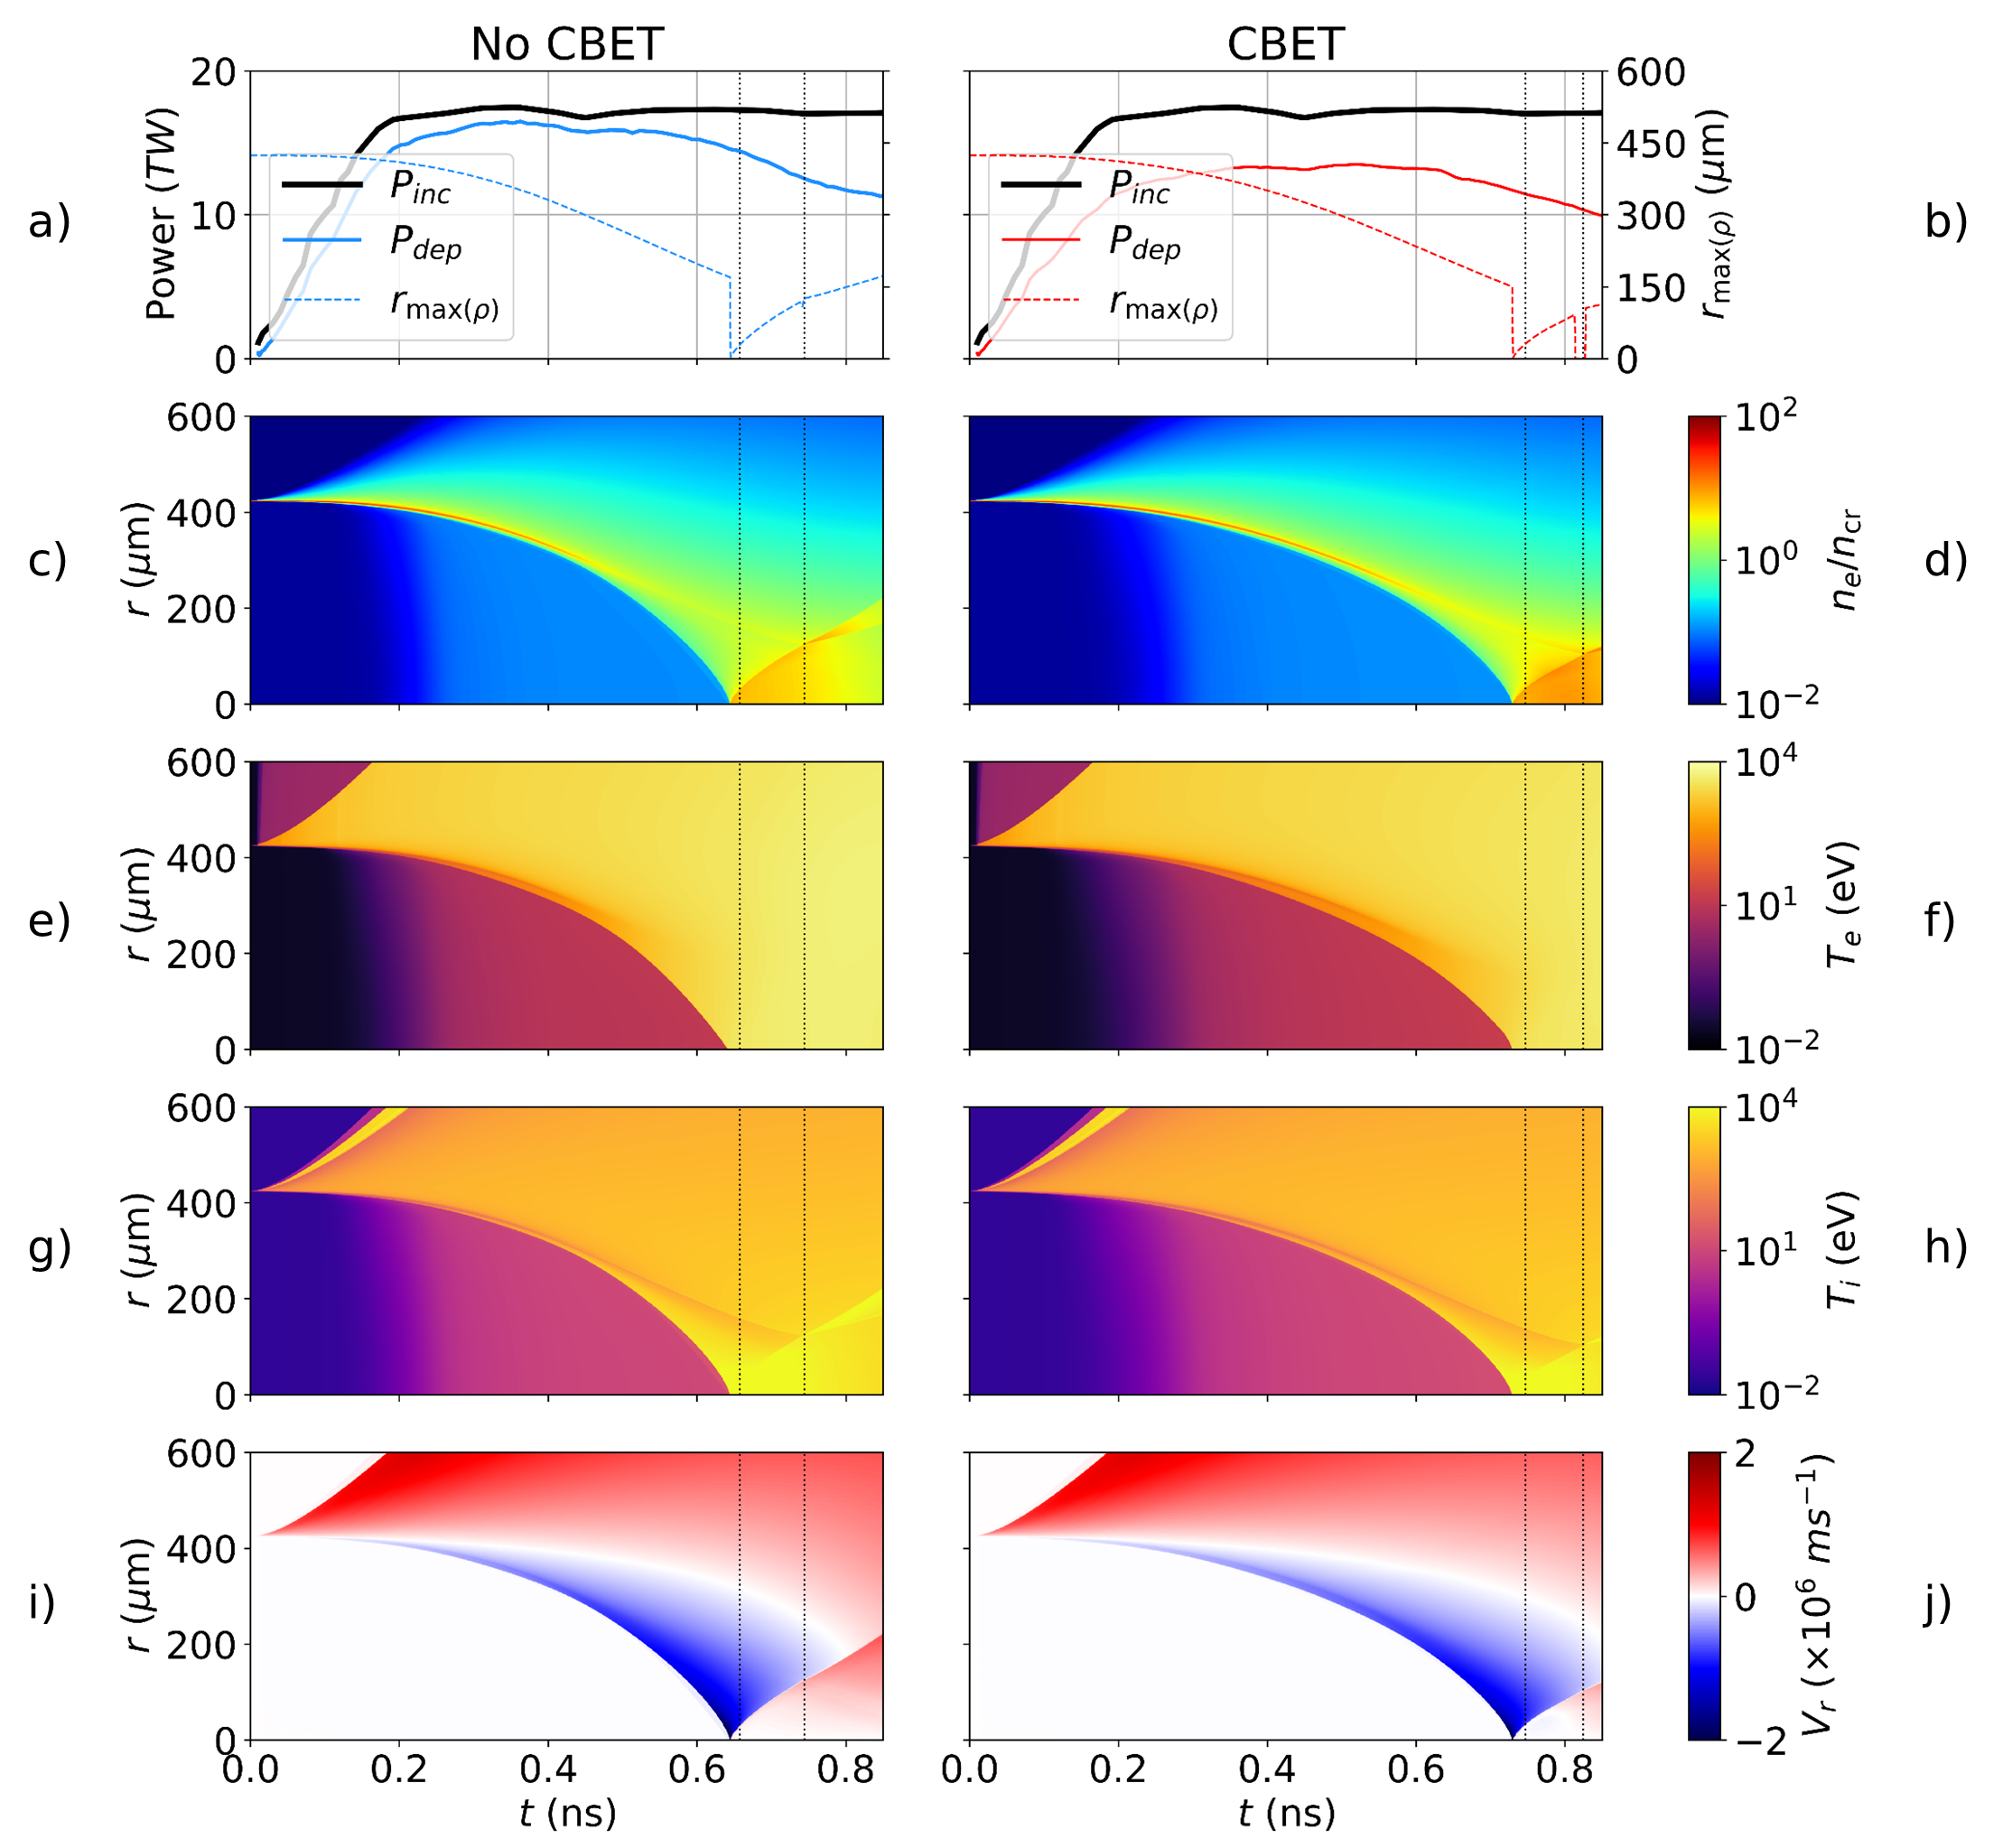
\includegraphics[width=\linewidth]{Results2/Images/expl_streaks.png}
    \centering
    \caption{1-D Simulation results both without (left) and with (right) \ac{CBET}.
    The top row plots the incident and absorbed energy from the simulation on the left axis and the radius of maximum density on the right.
    In order, the next rows plot $n_e$, $T_e$, $T_i$ and $V_r$.
    The full-width half-maximum times of the D${}_{2}$ yield are plotted as dotted vertical black lines on all panels.}%
    \label{fig:Res2_expl_streaks}
\end{figure}

Absorbed laser power as a function of time from these two simulations along with streak plots of hydrodynamic variables are plotted in Fig.~\ref{fig:Res2_expl_streaks}.
The left column of panels is from the no-\ac{CBET} simulation and the right are from the \ac{CBET} simulation.
The top row demonstrates that \ac{CBET} reduced the absorbed power by $\sim15\%$ during the implosion phase, up to about $t\sim0.6\ \text{ns}$.
Total absorbed laser energy was reduced from $81.1\%$ to $69.7\%$, from the no-\ac{CBET} to the \ac{CBET} simulation.
This reduced deposition, led to a slower and weaker shock being driven ahead of the imploding $\text{SiO}_2$ material, which is most clearly visible in the fourth panel, plotting $T_i$ on a log scale.
\ac{CBET} reduced the speed of the shock, such that it hit the axis for the with-\ac{CBET} simulation at $t\sim0.73\ \text{ns}$ compared to $t\sim0.65\ \text{ns}$ without \ac{CBET}.
Bangtime occurred for both simulations after this `shock-flash', as the rebounding Deuterium fuel compressed against the in-falling shell, creating thermonuclear densities.
Greater densities are observed for the with-\ac{CBET} simulation at bangtime, because the in-falling shell collides the rebounding shock at a smaller radius, \textit{i.e.} the shock timing of the implosion is better.
This somewhat compensated for the lower $T_i$ values due to the weaker shock, but overall, the no-\ac{CBET} simulation still produced a $\sim10\%$ higher neutron yield.
Note, that the effect of the fictitious, $Z=0$ material, that was placed outside the capsule to speed up the super-time-stepping thermal conduction routine, is visible from the large $T_i$ on the outer radius boundary of the expanding coronal plasma, which left the plot bounds at $t\sim0.2\ \text{ns}$.
Although not presented here, 1-D simulations with vacuum outside the glass ablator initially, showed minimal difference in bangtime hydrodynamic conditions and therefore integrated diagnostics.
Thus, the substantially faster configuration with the fictitious `vacuum' material was used for all 2-D simulations.

Compared to the streak plot of a more conventional, hotspot ignition implosion in Fig.~\ref{res1:Res1_streaks}, clear differences can be seen.
Firstly, the simulations presented in Fig.~\ref{res1:Res1_streaks} did not include radiation transport, which is the origin of the preheat ahead of the shock\footnote{\textit{i.e.} The temperature increase, which is visible in $T_e$ and $T_i$ plots, which hit the axis at $t\sim0.2\ \text{ns}$.} in Fig.~\ref{fig:Res2_expl_streaks}.
Secondly, the hotspot ignition design maintained a cold dense shell throughout the implosion phase, whereas the initially thin shell of the exploding-pusher simulation was approximately volumetrically heated.
Therefore, relatively little mass was left in the glass shell when the rebounding shock collided with it.
Finally, the $T_i$ increase in the exploding-pusher design was predominantly from the spherical convergence of the strong shock, compared to the stagnation heating in the hotspot design, which was localised to inside the decelerating shell when it compressed on axis, at $t\sim2.5\ \text{ns}$ in Fig.~\ref{fig:Res1_streaks}.
The lack of the cold dense shell is the reason that the exploding-pusher design cannot scale to high yield, because they have insufficient areal density to confine $\alpha$ particles and thus sustain a burn wave.

%################################################################################
%################################################################################
\subsection{2-D Simulations}%
\label{sec:Res2_expl2D}

\begin{figure}[t!]
    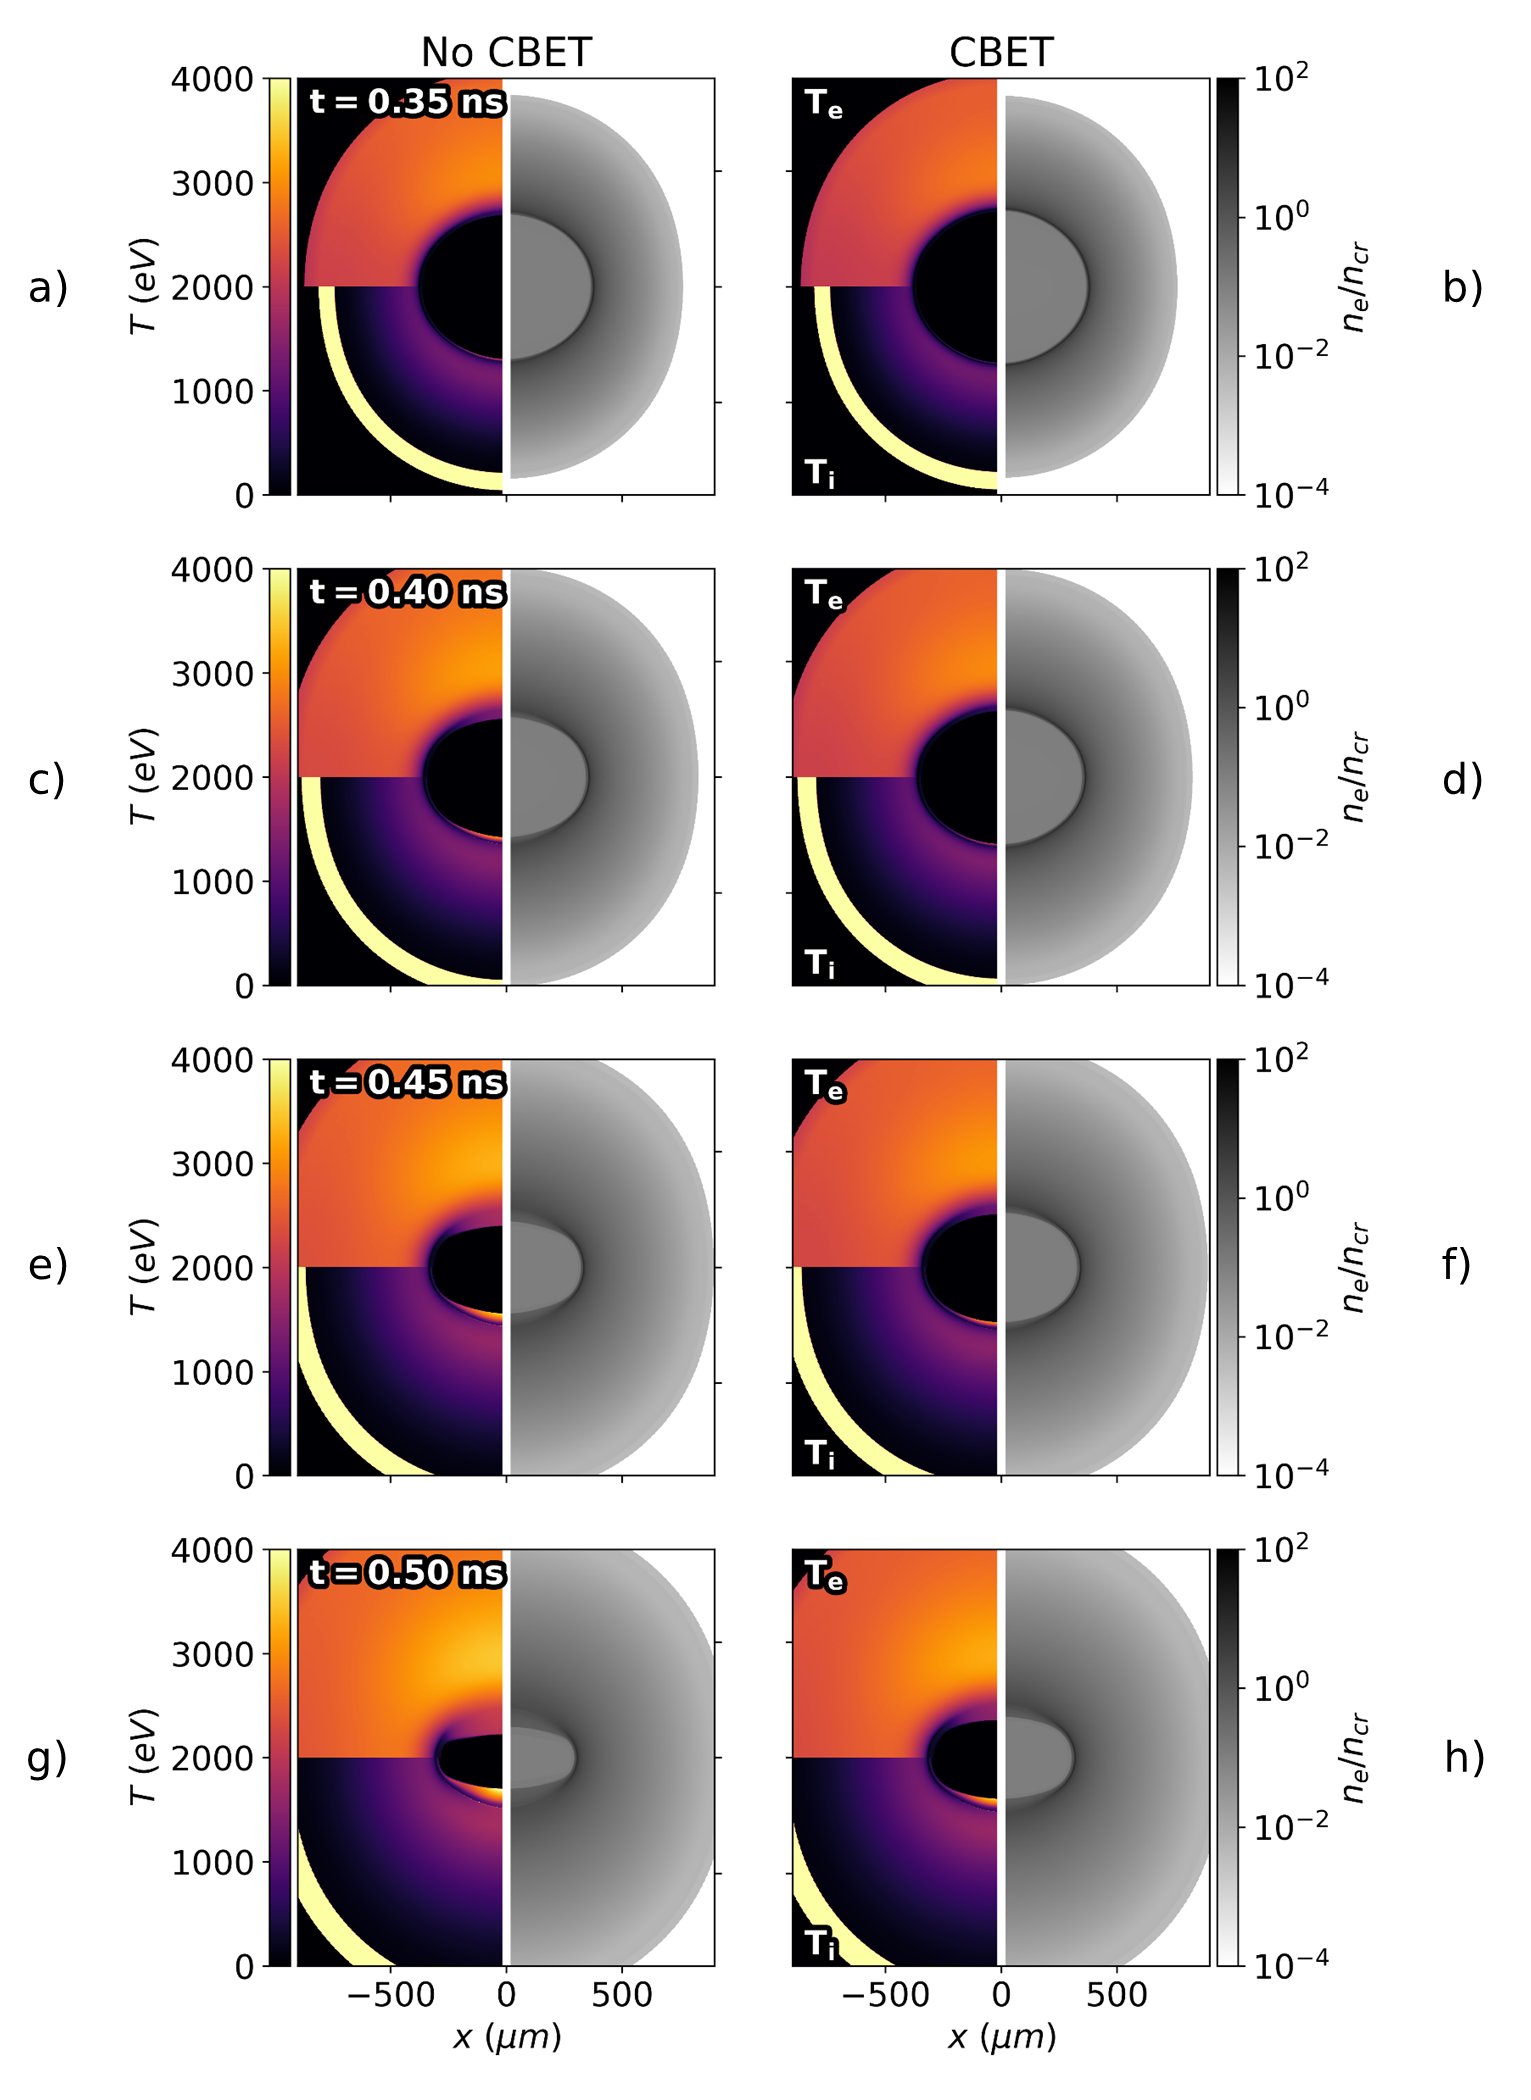
\includegraphics[width=0.95\linewidth]{Results2/Images/unmag_CBET_onoff.png}
    \centering
    \caption{$n_e$ (right-side), $T_e$ (top-left-side) and $T_i$ (bottom-left-side) plots from the 2-D, $0\ \text{T}$ simulations without (left-column) and with (right-column) \ac{CBET} at a variety of in-flight times.
    The decreased deposited energy due to \ac{CBET}, results in lower coronal electron temperatures and therefore a slower, weaker shock being driven, which is especially evident at later times.}%
    \label{fig:Res2_unmag_CBET_onoff}
\end{figure}

Simulations of this target configuration were also conducted in 2-D to explore how the non-uniformity of the laser-drive affected the implosion, both with and without \ac{CBET}.
2-D simulations used a 3-D \textsc{Solas} mesh to resolve the beam overlap pattern, with 58 cells in the azimuthal direction.
Fig.~\ref{fig:Res2_unmag_CBET_onoff} provides plots, which illustrate the progression of the simulation during the drive-phase.
The left column plots $T_e$, $T_i$ and $n_e$ from the 2-D, $B_{z0}=0\ \text{T}$ simulation without \ac{CBET}.
Integrated results from this simulation are given in the row labelled run 3 in Tab.~\ref{tab:Res2_magexpl_results}.
The right column plots the same for the equivalent simulation, but with the full effect of \ac{CBET} included, which corresponds to the row labelled run 5 in Tab.~\ref{tab:Res2_magexpl_results}.
Note that the viscous ion-heating of the fictitious material placed outside the glass shell initially, is again visible as large ion temperature in the layer immediately outside the coronal plasma expansion.

Particularly at the later times plotted in Fig.~\ref{fig:Res2_unmag_CBET_onoff}, the decreased, coronal $T_e$ of the \ac{CBET} compared to the no-\ac{CBET} simulation is visible.
The lower $T_e$ was due to of reduced absorption, because of \ac{CBET} scattering, and led to the shock from the no-\ac{CBET} simulation imploding significantly faster than the \ac{CBET} shock.
Thus, the no-\ac{CBET} implosion was more oblate during the drive-phase, because the shock travelled primarily along the $\hat{\vec{z}}$-axis, due to the beam-geometry.
However, when including \ac{CBET}, the velocity of the shock was reduced more than the velocity of the imploding portion of the glass shell, \textit{i.e.} $|V_{r,\text{shock}} - V_{r,\text{shell}}|$ was larger for the no-\ac{CBET} simulation than the \ac{CBET} simulation.
Therefore, the no-\ac{CBET} shock, after rebounding from the axis, collided with the shell and underwent maximal neutron production at a larger radius than for the \ac{CBET} result.
Thus, the oblateness parameter at bangtime in Tab.~\ref{tab:Res2_magexpl_results}, $(R_{\text{equator}}/R_{\text{pole}})|_{t=t_b}$, is significantly larger for the \ac{CBET} calculation.

Both 2-D simulations exhibited substantially reduced burn-averaged ion temperatures, compared to their 1-D equivalents.
This was primarily due to the strong shock travelling mainly along $\hat{\vec{z}}$, rather than radially inward as for the 1-D calculations.
Therefore, the convergence of the shock was reduced, leading to lower temperatures, and therefore neutron yields.
This interpretation is also corroborated by the increased $\Delta_b$ of all 2-D calculations compared to 1-D.
The burn-width was larger, because thermonuclear conditions were produced at different times throughout the hot fuel, as the rebounding $\text{D}_2$ compressed against the infalling shell material, compared to the 1-D where it was spherically symmetric.

In summary of these unmagnetised implosions in 1-D and 2-D, it has been shown that \ac{CBET} substantially reduced the deposited power for these exploding-pusher calculations.
1-D spherical calculations, which averaged the deposited power across all angles, demonstrated that this substantially reduced deposition led to a weaker shock being driven, which reduced thermonuclear yield and delayed the bangtime.
When 2-D effects were included, which better reflected the geometry of the laser-drive, this resulted in an oblate implosion, which reduced the convergence of the shock, and therefore the ion temperatures.
The reduced drive in the \ac{CBET} calculations also slowed the shock speed more than the infalling material, so the oblateness at bangtime (when the rebounding shock collided with the in-falling material) was greater when including \ac{CBET}.

%###############################################################################################################################
%###############################################################################################################################
%###############################################################################################################################
\section{Magnetisation in Exploding-Pusher Implosions}%
\label{sec:Res2_mag_unmag}

This section presents the effect that various extended-\ac{MHD} terms had on the magnetised, 2-D exploding-pusher simulations.
Simulations were conducted with an initial field strength $B_{z0}=\ 25\text{T}$ and particular terms turned off, to deduce what the important physical processes were.
The origin of the field structure is presented, which demonstrates that in the plasma corona, field lines are mainly radial due to the field being frozen in to highly conductive, radially outflowing plasma.
Anisotropic thermal conduction in this highly magnetised coronal plasma acted to keep heat localised to the polar regions, which enhanced the drive on the pole relative to the waist.
The results demonstrate that resistive diffusion and the Lorentz force have very little impact on the implosion physics, due to the bulk of the plasma being highly resistive and high-$\beta$ respectively.
Nernst-advection of the magnetic field acted to significantly redistribute the field in the low Hall parameter, equatorial region of the capsule, which formed a `divot' in density on the capsule waist.
This divot was however well separated from the region where burn was important, and thus had minimal impact on integrated neutron diagnostics.

%################################################################################
%################################################################################
\subsection{In-Flight Field Structure}%
\label{sec:Res2_field_structure}

\begin{figure}[t!]
    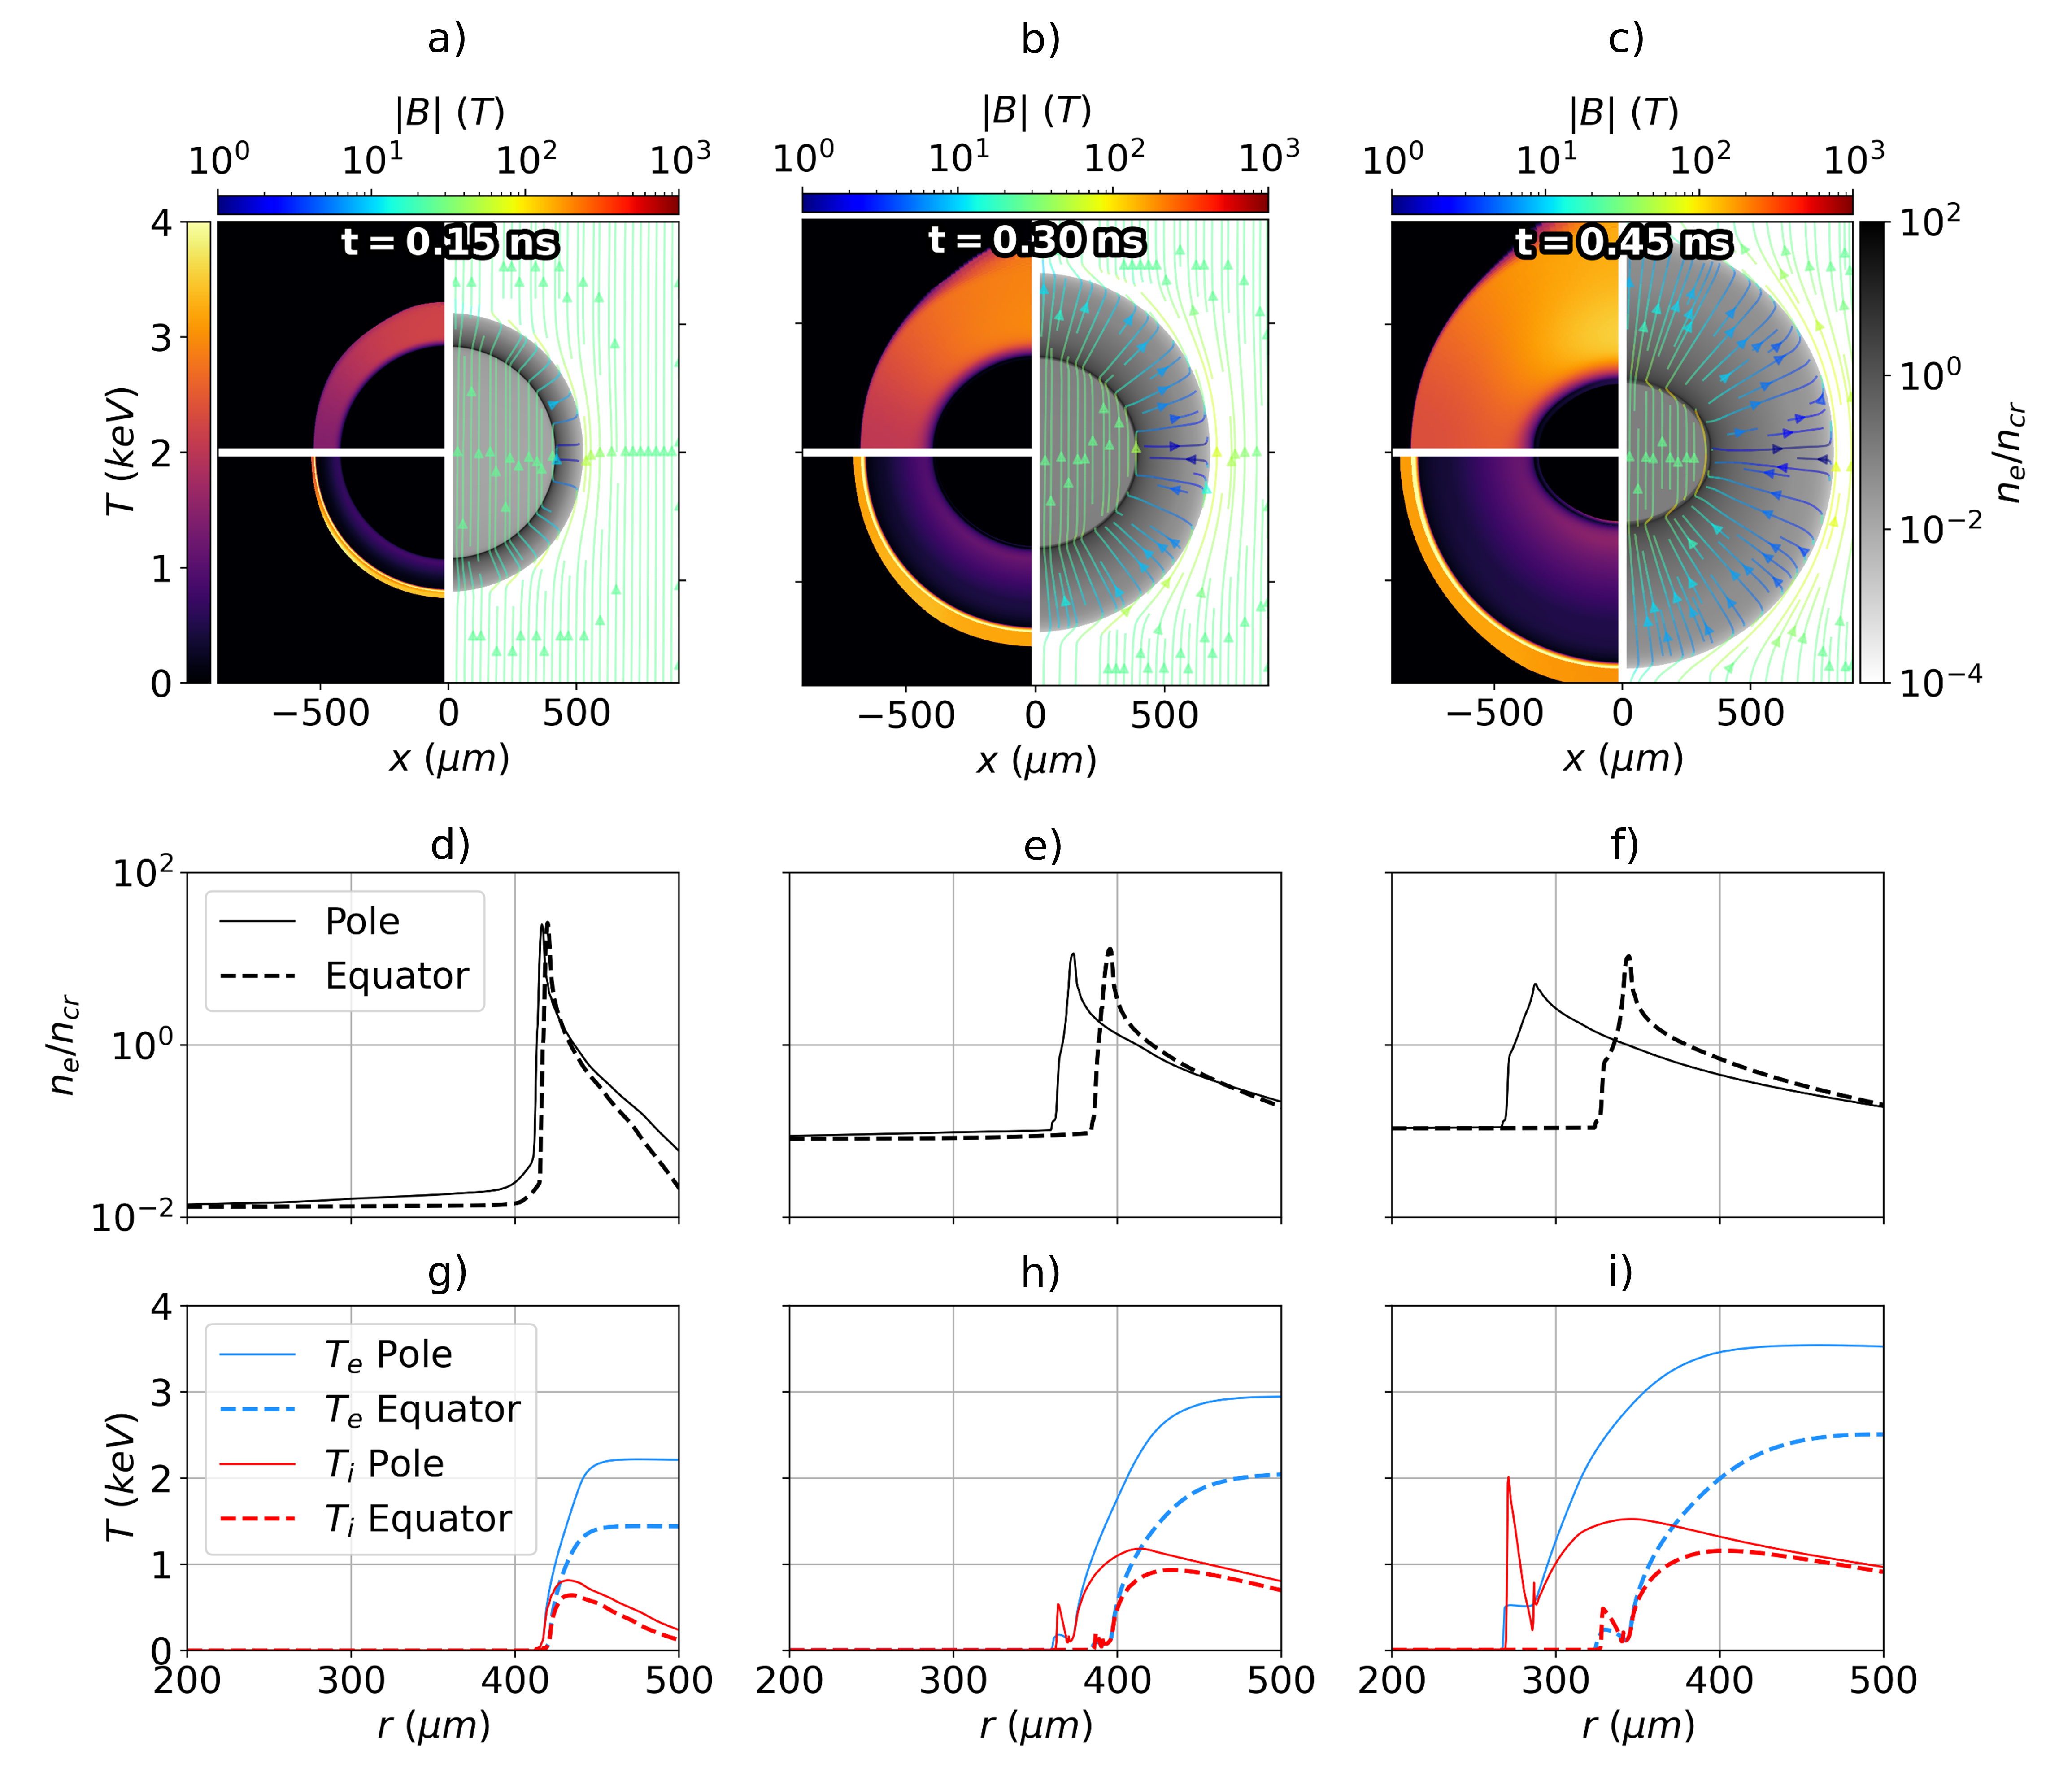
\includegraphics[width=\linewidth]{Results2/Images/mag_early_B_develop.png}
    \centering
    \caption{The development of the hydrodynamic variables and magnetic field structure from the $B_{z0}=25\ \text{T}$, \ac{CBET} simulation.
    Panels a), b) and c) plot $T_e$ (top-left), $T_i$ (bottom-left), $n_e$ (right) and $\vec{B}$ (streamlines) at $t=0.15$, $0.30$ and $0.45\ \text{ns}$ respectively.
    The approximately radially outward flowing, hot (and therefore highly conductive) ablating plasma pulled the magnetic field with it, resulting in radial $\vec{B}$ field lines, which were weaker at the capsule equator.
    Panels d), e) and f) plot $n_e$ lineouts along the pole ($\theta=0^{\circ}$) and equator ($\theta=90^{\circ}$).
    Panels g), h) and i) plot equivalent $T_e$ and $T_i$ lineouts.
    These all show that the increased polar temperatures, partially due to beam geometry and partially due to magnetisation, led to preferential ablation along the pole.}%
    \label{fig:Res2_mag_early_B_develop}
\end{figure}

Initially, the development of the coronal field structure from the $B_{z0}=25\ \text{T}$, no-\ac{CBET} simulation (labelled as run 5 in Tab.~\ref{tab:Res2_magexpl_results}) is presented.
The top row of Fig.~\ref{fig:Res2_mag_early_B_develop}, plots the drive phase hydrodynamic profiles, overlaid with streamlines of the magnetic field, coloured by its magnitude, at 3 different times.
Lineouts of $n_e$ and the temperatures are plotted in the middle and bottom rows respectively, along both the polar and equatorial directions.
The hot coronal plasma was highly conductive, shown explicitly in Sec.~\ref{sec:Res2_resis}, and thus the field remained frozen in to the plasma.
As the coronal plasma expanded outward therefore, it dragged the field lines with it, leading to $\vec{B}\sim\pm|\vec{B}|\hat{\vec{r}}$ in this, laser-heated region.
The geometric stretching of the field lines at the target poles was less significant than at the equator, and therefore the coronal field strengths were smallest at the target equator and highest on the poles.
As the target began to implode, the field compressed on the interior edge of the dense shell, resulting in non-radial field lines and an increase in field strength.
This effect is most clearly visible at $t=0.45\ \text{ns}$, in Fig.~\ref{fig:Res2_mag_early_B_develop}.c in the vicinity of the dense shell material region.

The lineouts clearly demonstrate that the preferential heating of the target on the pole, led to faster ablation of the shell along this direction.
This led to a much stronger shock along the pole, which is seen most clearly by the discrepancy in ion temperature between the pole and equator at $t=0.45\ \text{ns}$ in Fig.~\ref{fig:Res2_mag_early_B_develop}.i.
Increased polar electron temperature is partially due to the pole heavy drive from the beam geometry, and also due to anisotropic thermal conduction.
The field structure plotted in Fig.~\ref{fig:Res2_mag_early_B_develop}, inhibited equilibration of temperature via thermal conduction in the polar direction, which increased the temperature asymmetry compared to the unmagnetised simulation.
Anisotropic thermal conduction and its impact in this configuration is discussed in more detail in Sec.~\ref{sec:Res2_aniso}.

%################################################################################
%################################################################################
\subsection{Resistive Diffusion and the Lorentz Force}%
\label{sec:Res2_resis}

\begin{figure}[t!]
    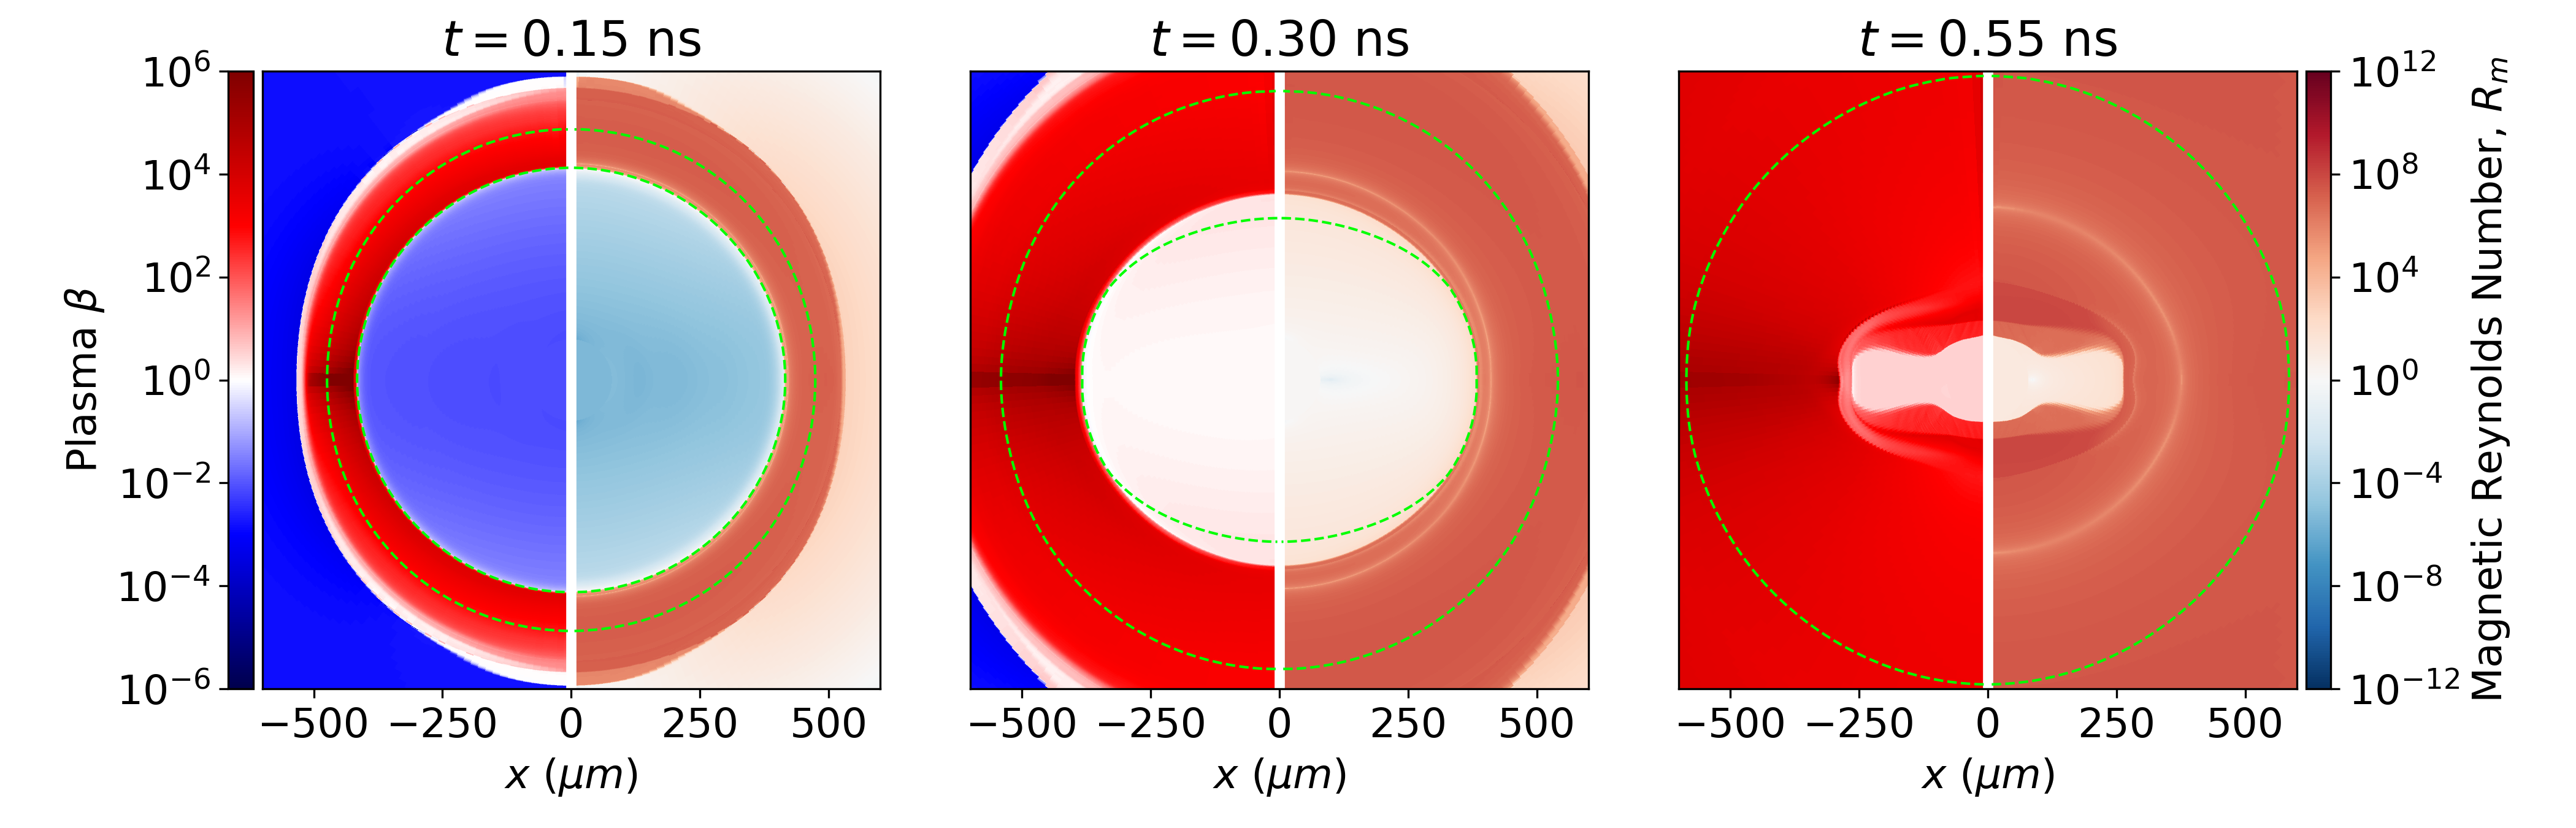
\includegraphics[width=\linewidth]{Results2/Images/magmag_beta_Rm.png}
    \centering
    \caption{Plasma $\beta$ (left-side) and Magnetic Reynolds Number, $R_m$, (right-side) at various in-flight times, throughout the $B_{z0}=25\ \text{T}$, no-\ac{CBET} simulation.
    Contours of the $n_e=n_{cr}/10$ are plotted on all panels as dashed green lines to indicate the bounding region, which contained a significant amount of plasma.
    Broadly, the $\beta$ and $R_m$ values are $\gg 1$ in all regions with an appreciable amount of material, which demonstrates that the Lorentz force and resistive diffusion should have minimal effect on the implosion dynamics.}%
    \label{fig:Res2_magmag_beta_Rm}
\end{figure}

As was stated in the above Sec.~\ref{sec:Res2_field_structure}, the coronal plasma was highly conductive for all simulations, due to the combination of high temperature and relatively low density.
The right side of each panel Fig.~\ref{fig:Res2_magmag_beta_Rm} plots the Magnetic Reynolds Number, $R_m$, at three times during the implosion of the $B_{z0}=25\ \text{T}$, no-\ac{CBET} simulation, labelled as run 6 in Tab.~\ref{tab:Res2_magexpl_results}.
As was stated in Sec.~\ref{sec:theory_mag_theory}, $R_m$ is the ratio of magnetic field advection to diffusion.
Conservatively, a $1\ \mu\text{m}$ length scale was used to calculate this value, which was approximately the smallest length scale observed throughout the implosion across all times.
Thus, for the majority of the simulation, $R_m$ is likely underestimated, because $R_m\propto L$.
The green dashed lines are contours of $n_e=n_{\text{cr}}/10$, which are included in the plots to illustrate the regions of the simulation that contained the majority of the plasma material.
Although Fig.~\ref{fig:Res2_magmag_beta_Rm}.a shows that early in the simulation, the gas fill of the capsule had a small value of $R_m$, and therefore resistive diffusion dominated over frozen in flow, the dynamics of the implosion had not reached this region yet, \textit{i.e.} it is not bounded by the $n_e$ contours.
The radiative preheat also raised the temperature, and therefore $R_m$ value in this region, before the time plotted in Fig.~\ref{fig:Res2_magmag_beta_Rm}.b.
Therefore, the majority of the plasma material had a high value of $R_m$ throughout the implosion, mainly due to the high temperatures, demonstrating that frozen-in-flow dominated over resistive diffusion.
This is corroborated by comparing run 6 and run 15 in Tab.~\ref{tab:Res2_magexpl_results}, which did not include the effects of resistive diffusion on the field transport.
There is minimal difference across all metrics between these two rows, which shows that the global dynamics of both simulations were very similar.

The left side of the panels in Fig.~\ref{fig:Res2_magmag_beta_Rm} plots the plasma $\beta$ at the same times for the same simulation.
As was stated in Sec.~\ref{sec:theory_mag_theory}, this is the ratio of thermal plasma pressure to magnetic pressure and thus describes whether thermal forces or the Lorentz force, is likely to predominantly influence the plasma dynamics.
Just as was seen for $R_m$, the value of this parameter was generally high in all regions with appreciable plasma density throughout the implosion, so the Lorentz force was assumed to minimally influence the plasma dynamics.
An additional simulation was performed, in which the effect Lorentz force was not included on the plasma, labelled by run 13 in Tab.~\ref{tab:Res2_magexpl_results}.
Again, there is minimal difference in integrated metrics between this and run 6 (the comparable run which included the Lorentz force), which verifies this analysis.

%################################################################################
%################################################################################
\subsection{Anisotropic Thermal Conduction}%
\label{sec:Res2_aniso}

\begin{figure}[t!]
    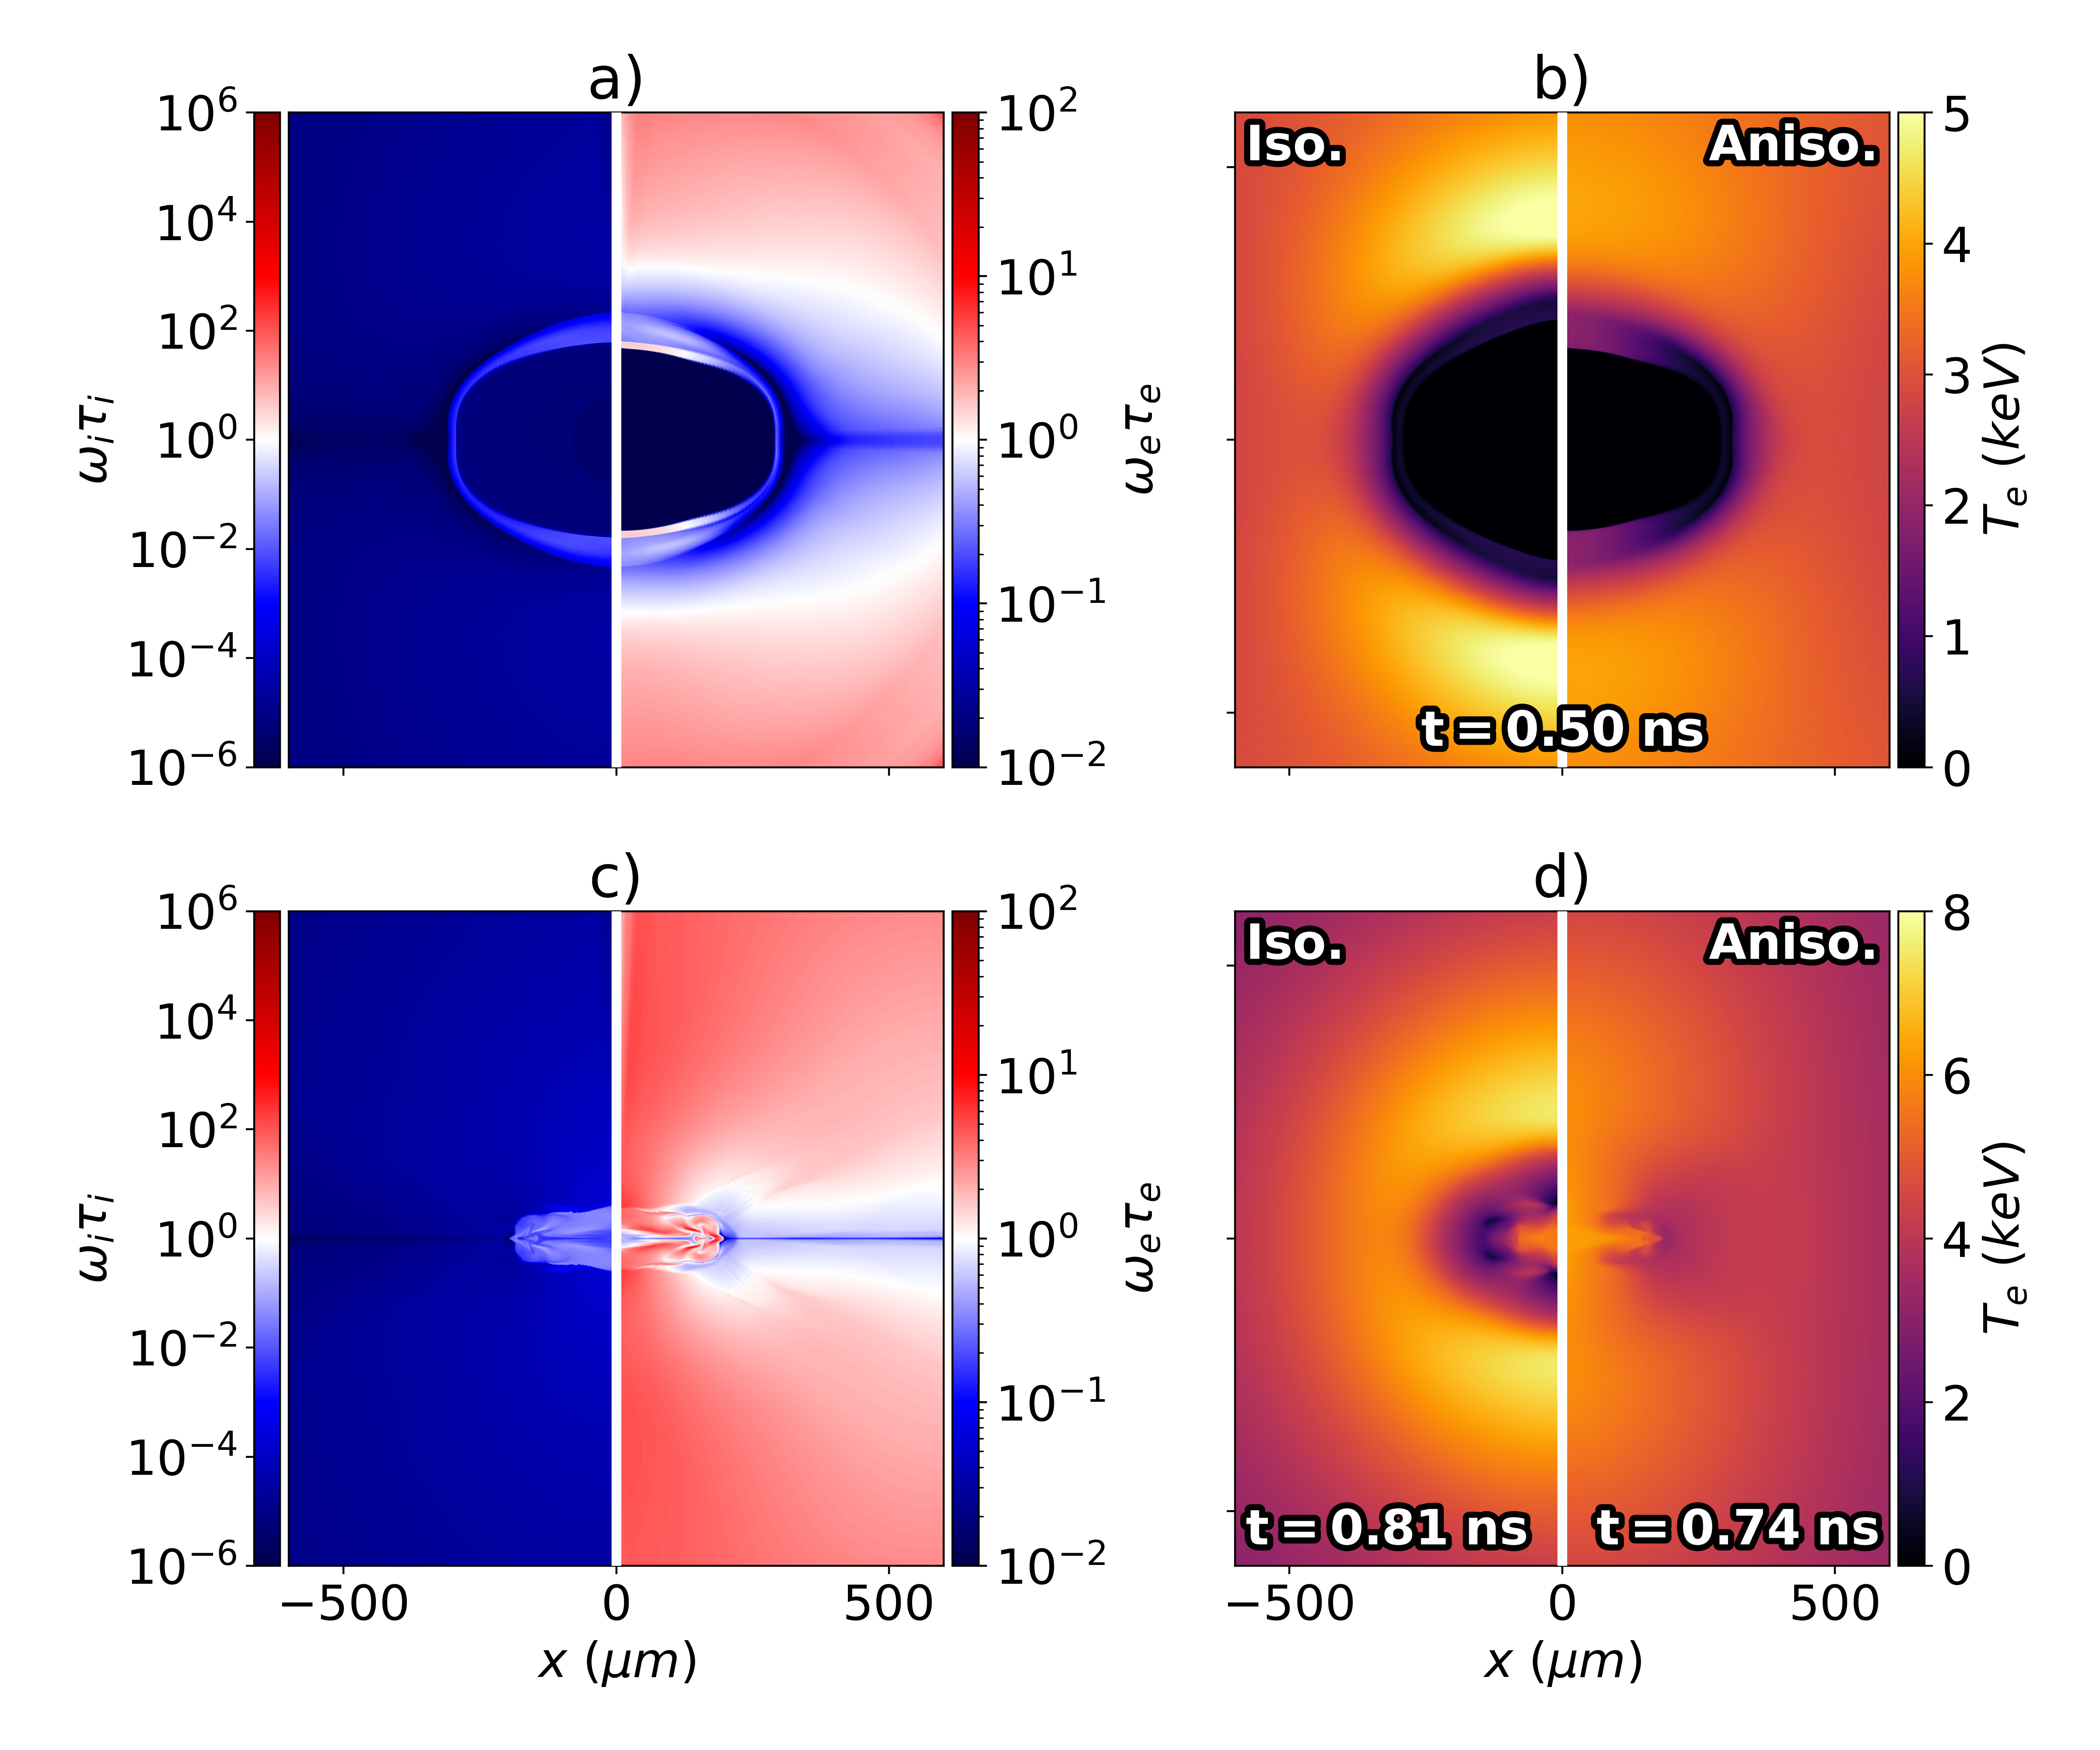
\includegraphics[width=0.8\linewidth]{Results2/Images/iso_aniso.png}
    \centering
    \caption{In-flight a) and bangtime c) Hall parameters, from the $B_{z0}=25\ \text{T}$, no-\ac{CBET} simulation.
    Panel b) plots the $T_e$ from the isotropically magnetised simulation (left-side) and anisotropic conduction simulation (right-side) in-flight.
    Panel d) plots the same, but at bangtime.
    The electron Hall parameter was $>1$ at the poles due to high magnetic fields and temperatures, which led to significantly restricted thermal conduction from magnetised transport.
    Isotropically magnetised conduction, therefore resulted in a markedly different bangtime morphology, as is shown in panels b) and d).
    Ion hall parameters peaked at bangtime, when values reached about $\omega_i\tau_i\sim0.1$.}%
    \label{fig:Res2_iso_aniso}
\end{figure}

In order to understand the effect of anisotropic thermal conduction, an additional simulation was performed, which had the same setup as the $B_{z0}=25\ \text{T}$, no-\ac{CBET} simulation, but thermal conduction was isotropically suppressed by the local magnetic field strength, regardless of its orientation.
The anisotropic and isotropic simulations are labelled by run 6 and 12 respectively in Tab.~\ref{tab:Res2_magexpl_results}
Explicitly, the parallel conductivity was forced to take the value of the perpendicular conductivity, $\kappa_{\parallel}=\kappa_{\perp}$.
Comparison of this isotropically suppressed conduction simulation, with the $B_{z0}=25\ \text{T}$, no-\ac{CBET} simulation, elucidated the role of anisotropic conductivities relative to the orientation of the field.
Fig.~\ref{fig:Res2_iso_aniso}.a plots the ion (left-side) and electron (right-side) hall parameters from the $B_{z0}=25\ \text{T}$, no-\ac{CBET}, anisotropic thermal conduction simulation at $t=0.5\ \text{ns}$.
It can be seen that the polar region of the corona was significantly magnetised, with $1<\omega_e\tau_e<10$, therefore thermal conduction in this region was significantly suppressed perpendicular to the field in the anisotropic simulation, which was approximately the polar direction, as is seen in Fig.~\ref{fig:Res2_mag_early_B_develop}.c.
Ion Hall parameters peaked at values of  $\omega_i\tau_i\sim10^{-2}$ in-flight, thus ion transport was not expected to be significantly affected by the field.

The electron temperature profiles at the same time are plotted in Fig. \ref{fig:Res2_iso_aniso}.b for the isotropically magnetised conduction simulation (left-side) and anisotropic simulation (right-side).
The $T_e$ profile of the anisotropic case was significantly more oblate than the isotropic simulation and the polar regions of the isotropic region were also significantly hotter.
This was due to decreased transport of deposited laser energy in the isotropic to the ablation region, because heat could not freely stream radially inward along the field lines when conductivity was isotropically suppressed by the field.
Isotropic magnetisation of electron transport thus led to reduced ablation at the poles and a larger critical radius along $\pm\hat{\vec{z}}$, which gave the implosion and shock a rounder shape.

Bangtimes temperature profiles, plotted in Fig.~\ref{fig:Res2_iso_aniso}.d, corroborate this analysis, which demonstrate that the isotropic simulation had a significantly rounder shape.
The oblateness parameter in Tab.~\ref{tab:Res2_magexpl_results}, obtained by fitting an ellipse to the radius of maximum density at bangtime, also demonstrates a less oblate profile.
By isotropically magnetising the conduction, $(R_{\text{equator}}/R_{\text{pole}})|_{t=t_b}$ was reduced from $3.80\rightarrow3.14$.
The reduced ablation coupled less energy to the implosion, evident in the reduced bangtime from $t_b=0.74\rightarrow0.81\ \text{ns}$, going from anisotropic to isotropic thermal conduction.
Yield still increased for the isotropic simulation from $4.72\rightarrow5.02\times10^{10}$, which shows that integrated yield metrics are a fine balance of many factors, including coupled energy and implosion shape.

The bangtime Hall parameters are plotted in Fig.~\ref{fig:Res2_iso_aniso}.c, which show highly magnetised electrons and moderately magnetised ions, with a maximum $\omega_i\tau_i\sim10^{-1}$.
Note that this is also for an initial field strength $B_{z0}=25\ \text{T}$ simulation.
For the $B_{z0}=50\ \text{T}$, with-\ac{CBET} simulation, which included \ac{CBET} fully and is therefore the most realistic simulation to compare with experiment at this field strength, the maximum ion Hall parameter was also $\omega_i\tau_i\sim10^{-1}$.
This is lower than the reported value of $\omega_i\tau_i\sim1$ in the original paper~\cite{bose_effect_2022}.
However, improved sphericity of the converging shock, which could change slightly for example by changing $f_{\text{lim},e}$, would markedly boost this value.
The hall parameter, $\omega\tau\propto T^{3/2}|\vec{B}|$, so a less oblate shock would increase the value this by both better flux compression of the field, and higher stagnation temperatures, due to greater convergence of the shock.

%################################################################################
%################################################################################
\subsection{The Nernst Effect}%
\label{sec:Res2_nernst}

\begin{figure}[t!]
    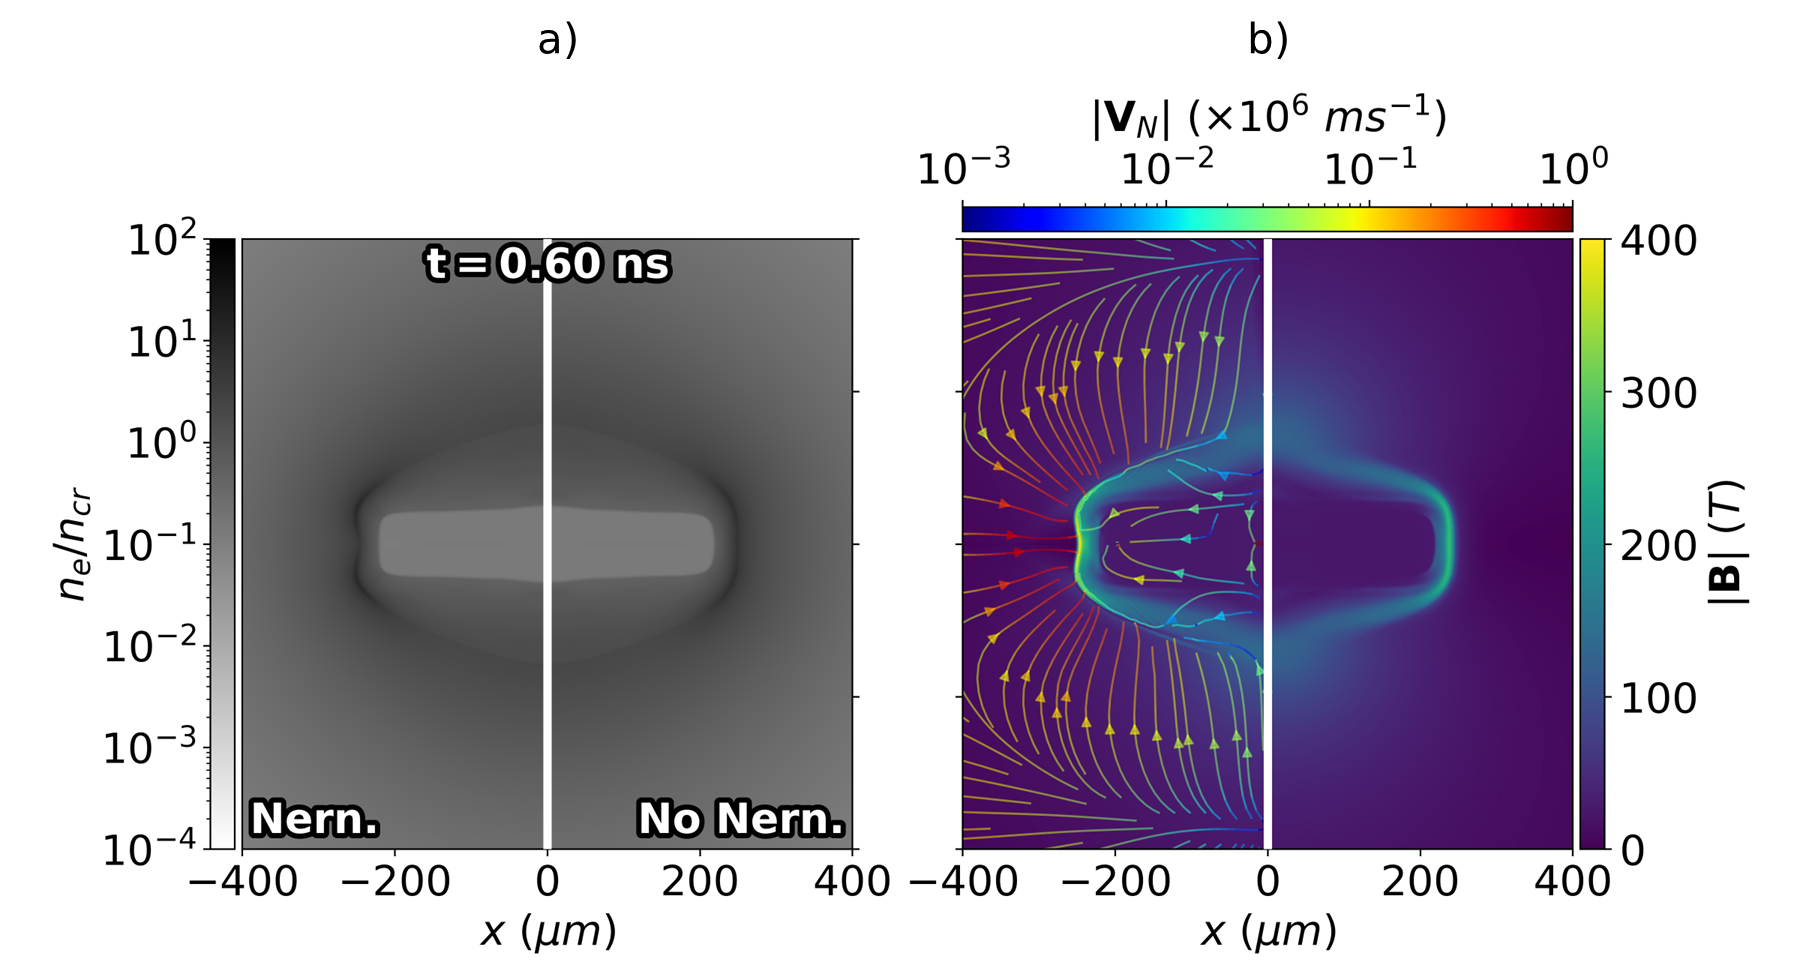
\includegraphics[width=\linewidth]{Results2/Images/nernst_comp_Bstream.png}
    \centering
    \caption{Panel a) plots in-flight electron density profiles from the $B_{z0}=25\ \text{T}$, no-\ac{CBET} simulations with (left-side) and without (right-side) Nernst advection of the magnetic field.
    The magnetic field is also plotted as streamlines in the top-half of each plot, coloured by magnitude.
    Panel b) plots magnetic field magnitude from the Nernst (left-side) and no-Nernst (right-side) simulation along with Nernst advection velocity streamlines from the Nernst-on simulation.
    Advection of the field is important in the low Hall parameter equatorial region, pulling $\vec{B}$ down $\nabla T_e$, into the dense wall.
    Altered field at the equator impacts on the magnetised thermal conduction, which ultimately imprints on the density, as is seen in panel a).}%
    \label{fig:Res2_nernst_comp}
\end{figure}

The final extended-\ac{MHD} term that was independently examined was the Nernst effect.
In \textsc{Chimera}, Nernst is implemented as an advection of $\vec{B}$ down $\nabla T_e$~\cite{walsh_extended-magnetohydrodynamics_2020}.
It is a collisional term, and therefore dominates in plasma with low values of $\omega_e\tau_e$.
The plots of Hall parameter in Fig.~\ref{fig:Res2_iso_aniso} demonstrate that the coronal plasma has low Hall parameters at the equator, which suggests that the Nernst effect would be most important at the equator of the capsule and have minimal effect on the field profiles near the poles.
An additional simulation, with $B_{z0}=25\ \text{T}$ and no-\ac{CBET}, was conducted without Nernst advection of magnetic field to understand its impact upon the field and plasma dynamics.
The simulation without the Nernst effect is labelled in Tab.~\ref{tab:Res2_magexpl_results} as run 14.

Fig.~\ref{fig:Res2_nernst_comp}.b plots the magnetic field strength from equivalent simulations with-Nernst (left-side) and without-Nernst (right-side) at $t=0.60\ \text{ns}$.
The simulation including Nernst (run 6 in Tab.~\ref{tab:Res2_magexpl_results}), also plots the Nernst advection velocity as streamlines, coloured by the speed.
The largest advection speeds are $\sim10^6\ \text{ms}^{-1}$, which is comparable to the coronal fluid ablation speed, demonstrating that Nernst-advection is non-negligible in dictating the magnetic field structure.
As expected, the equator of the target had the largest Nernst speeds, due to the low Hall parameter, and it acted to push field from the coronal plasma onto the interior edge of the shell.
This created a localised field `pile-up' in this region for the Nernst simulation, compared to the simulation on the right.

Fig.~\ref{fig:Res2_nernst_comp}.a plots the electron density at the same time for the Nernst (left-side) and no-Nernst (right-side) simulations alongside magnetic field streamlines from the same simulations on the top-half of the plot.
The streamlines show that the Nernst effect caused the coronal field lines at the equator to be radial, by pushing $B_z$ down the mostly radial temperature gradient, towards the shell.
It is visible that the altered magnetic field structure impacted on the plasma density indirectly, creating an equatorial bump in the shell density, which is not present in the right-side plot without Nernst included.
This bump only appeared in simulations with both Nernst and anisotropic conduction, which shows that this altered field profile changed the anisotropic thermal conduction at the equator, which then impacted upon the density.
The effective re-orientation of $\vec{B}$ at the equator, meant that thermal conduction which transported laser energy from the deposition surface to the ablation surface, experienced the higher, parallel thermal conductivity $\kappa_{\parallel}$, rather than $\kappa_{\perp}$.
This locally increased the drive along $z\sim0$, leading to the bump at the equator.

Comparison of run 6 (Nernst) and run 14 (no-Nernst) in Tab.~\ref{tab:Res2_magexpl_results}, shows minimal difference in the integrated metrics, despite the altered dynamics.
This is mostly because the changes were localised to the equator, which was well separated from the polar region, which experienced the strongest shock convergence and therefore greatest temperatures and neutron production.
It is expected however, that experiments with symmetric laser illumination, and therefore a less oblate implosion, may be more influenced by the Nernst effect, because the equator of the shell would partake more in neutron production.
Additionally, it is worth noting that this bump is likely to only be observed in magnetised direct-drive implosion and not indirect-drive.
This is because the main action of Nernst in these simulations was to change the field and therefore anisotropic transport in the conduction zone, which is the layer in direct-drive implosions that transports energy from the laser absorption region to the ablation surface.
However, for indirect-drive, x-rays penetrate effectively all the way through to the ablation surface, so there is no conduction zone.
Thus, the altered conduction zone field profile would have a much less significant impact on the density for indirect-drive.

%###############################################################################################################################
%###############################################################################################################################
%###############################################################################################################################
\section{The Effect of Magnetisation on Cross-Beam Energy Transfer and Stagnation}%
\label{sec:Res2_mag_on_CBET}

\begin{figure}[t!]
    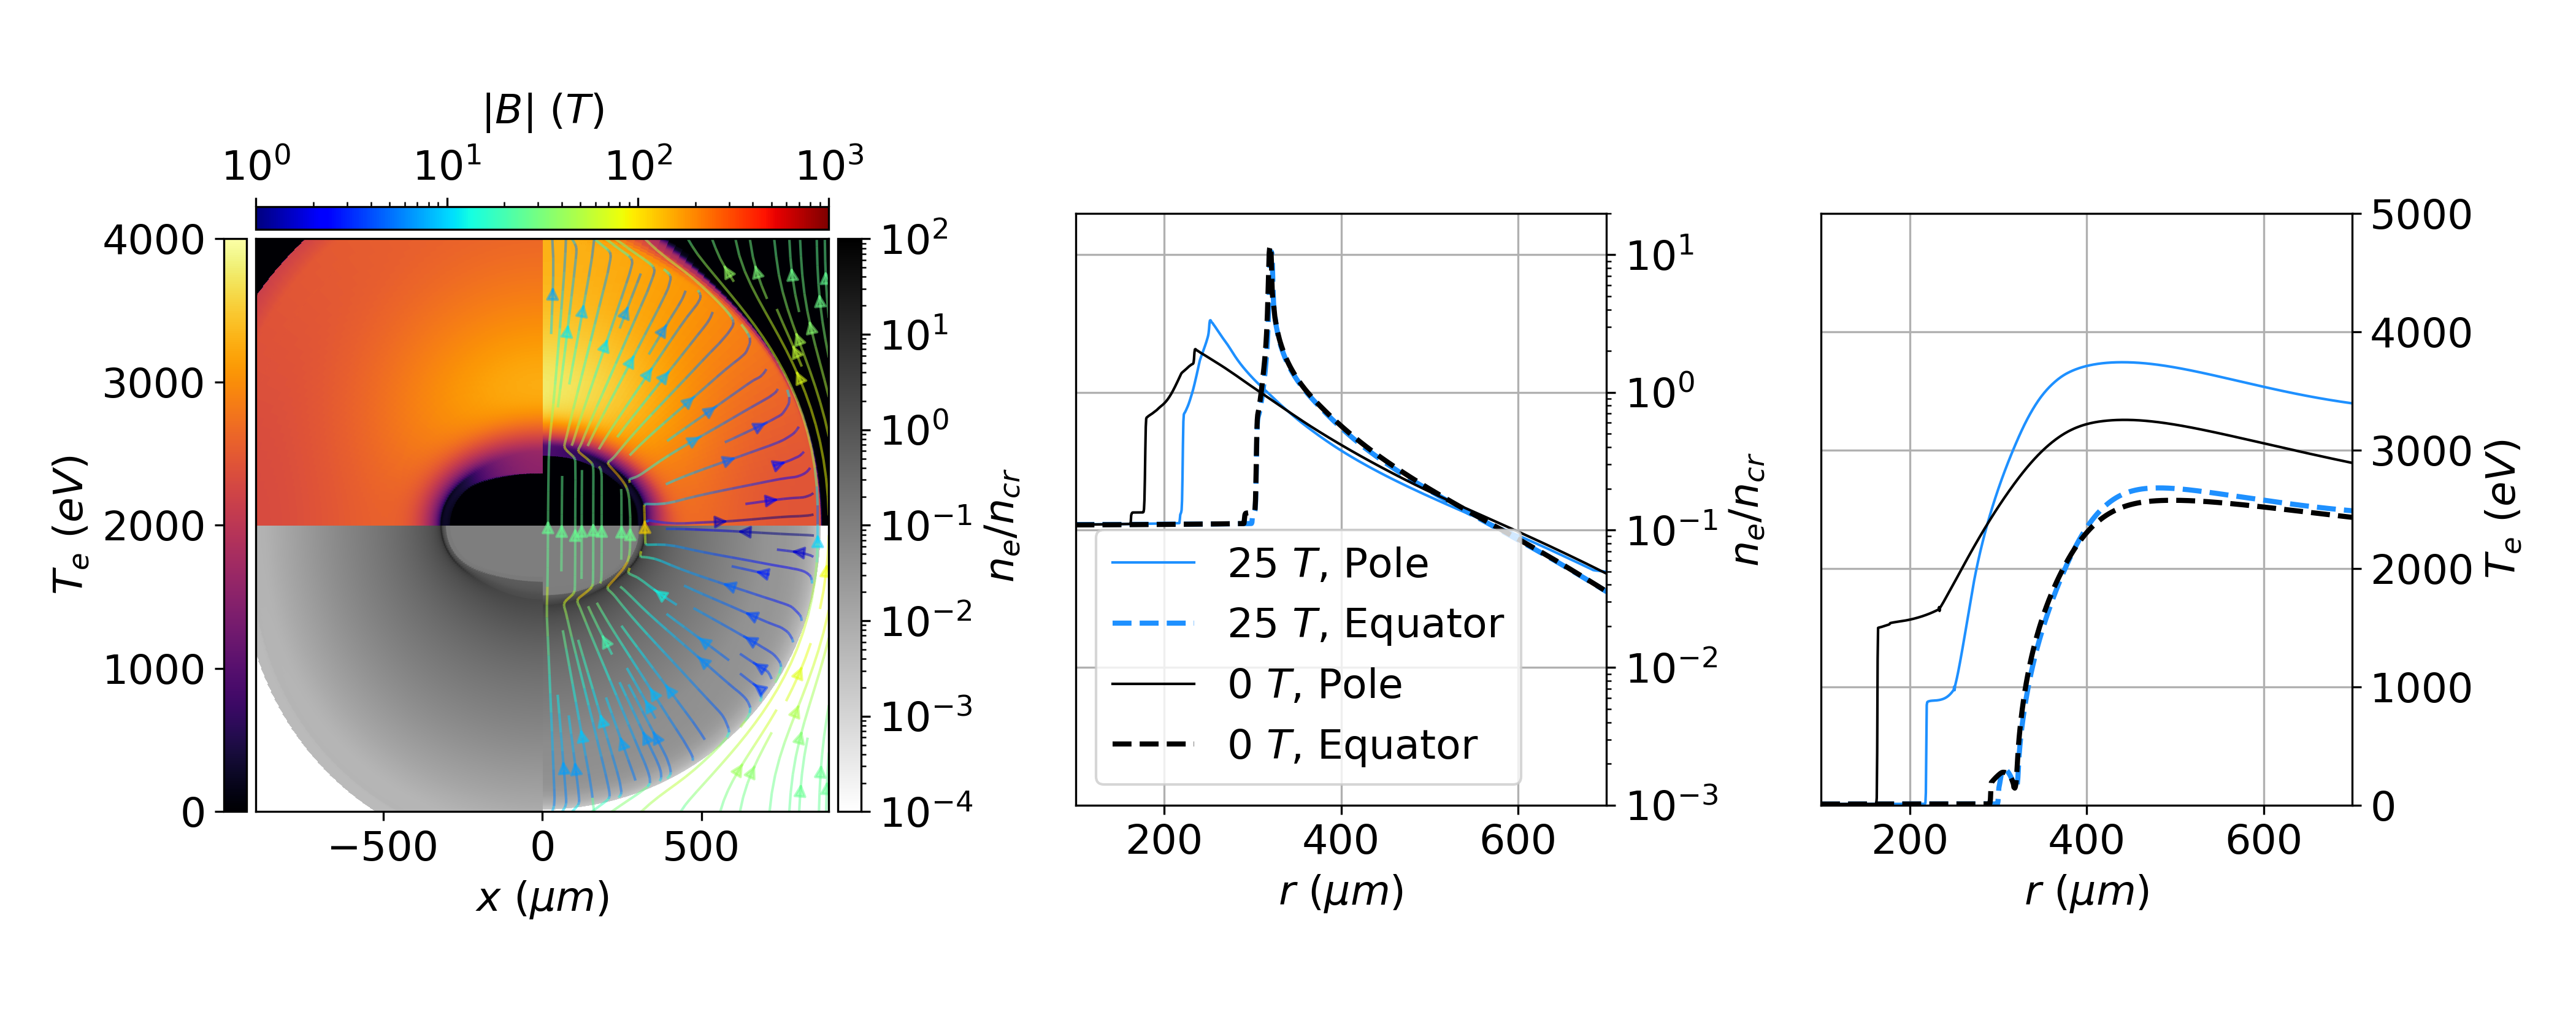
\includegraphics[width=\linewidth]{Results2/Images/ne_te_Bstream_comp_alt050.png}
    \centering
    \caption{Comparison of $n_e$ and $T_e$ profiles from the $B_{z0}=0$ (panel a) left-side) and $25\ \text{T}$ (panel a) right-side), with-\ac{CBET} simulations, both at $t=0.5\ \text{ns}$.
    Panel a) also plots streamlines of $\vec{B}$ for the $B_{z0}=25\ \text{T}$ simulation, coloured by the field magnitude.
    Panels b) and c) plot $n_e$ and $T_e$ lineouts respectively, along both the pole and equator.
    It is evident from these lineouts that magnetisation anisotropically affects hydrodynamic variables, which are used to calculate the \ac{CBET} gain.
    Therefore, it is anticipated that magnetisation could anisotropically affect the \ac{CBET} scattering volume.}%
    \label{fig:Res2_ne_te_Bstream_comp_alt050}
\end{figure}

This section presents results on how the magnetisation of the corona affects both \ac{CBET} scattering and the stagnation shape of the implosion.
Fig.~\ref{fig:Res2_ne_te_Bstream_comp_alt050}.a plots $T_e$ and $n_e$ from the $B_{z0}=0$ (left-side) and $25\ \text{T}$ (right-side), with-\ac{CBET} simulations at $t=0.5\ \text{ns}$.
Fig.~\ref{fig:Res2_ne_te_Bstream_comp_alt050}.b and Fig.~\ref{fig:Res2_ne_te_Bstream_comp_alt050}.c plot lineouts of $n_e$ and $T_e$ respectively, along both the poles and equator for both simulations.
As was shown in Sec.~\ref{sec:Res2_mag_unmag}, anisotropic thermal conduction is the dominant effect of magnetisation in these implosions.
The equatorial lineouts are similar, due to low Hall parameters in this region and thus minimal impact of magnetisation upon the transport.
However, the polar lineouts are significantly different in the magnetised and unmagnetised cases.
Magnetisation has amplified the $\ell=2$ asymmetry of the coronal plasma $n_e$ and $T_e$ profiles, which are used to calculate the \ac{CBET} gain.
It was therefore hypothesised, that this amplified asymmetry in coronal profiles due to magnetisation, would leave a signature upon the \ac{CBET} and therefore implosion dynamics, because \ac{CBET} is known to interact strongly with low mode, coronal asymmetries~\cite{anderson_effect_2020}.

In this chapter `partial-\ac{CBET}' simulations shall be presented, for which the coupled power as a function of time was kept the same as the equivalent with-\ac{CBET} simulation, \textit{i.e.} so \ac{CBET} only acted to reduce the magnitude of the deposited power, rather than redistribute it around the target.
It was hoped that, by comparison with the full-\ac{CBET} simulations, this would demonstrate that \ac{CBET} changed the shape of the implosion differently, for different levels of seed magnetic field.
The results presented in this section demonstrate that the $\ell=2$ of the long-wavelength, density perturbation was slightly reduced by \ac{CBET}, consistent with existing literature on how \ac{CBET} mitigates $\ell=1$ asymmetries~\cite{colaitis_inverse_2021}.
Results also showed that the increasingly anisotropic coronal plasma profiles for increasing seed magnetic field strengths, did lead to changes in the \ac{CBET} scattering.
However, this was too small an effect to lead to experimentally observable changes in density and temperature.
It is hypothesised that the polar beam geometry, the shock driven characteristics of the exploding-pusher implosions and the high $Z$ shell (which results in increased coronal temperatures, and therefore reduced \ac{CBET}~\cite{colaitis_exploration_2023}), minimised the impact on \ac{CBET} scattering.
Suggestions for an alternative implosion are provided, which would increase the likelihood of an experimentally observable signature.

%################################################################################
%################################################################################
\subsection{Analysis and Key Definitions}%
\label{sec:Res2_analysis_definitions}

\begin{figure}[t!]
    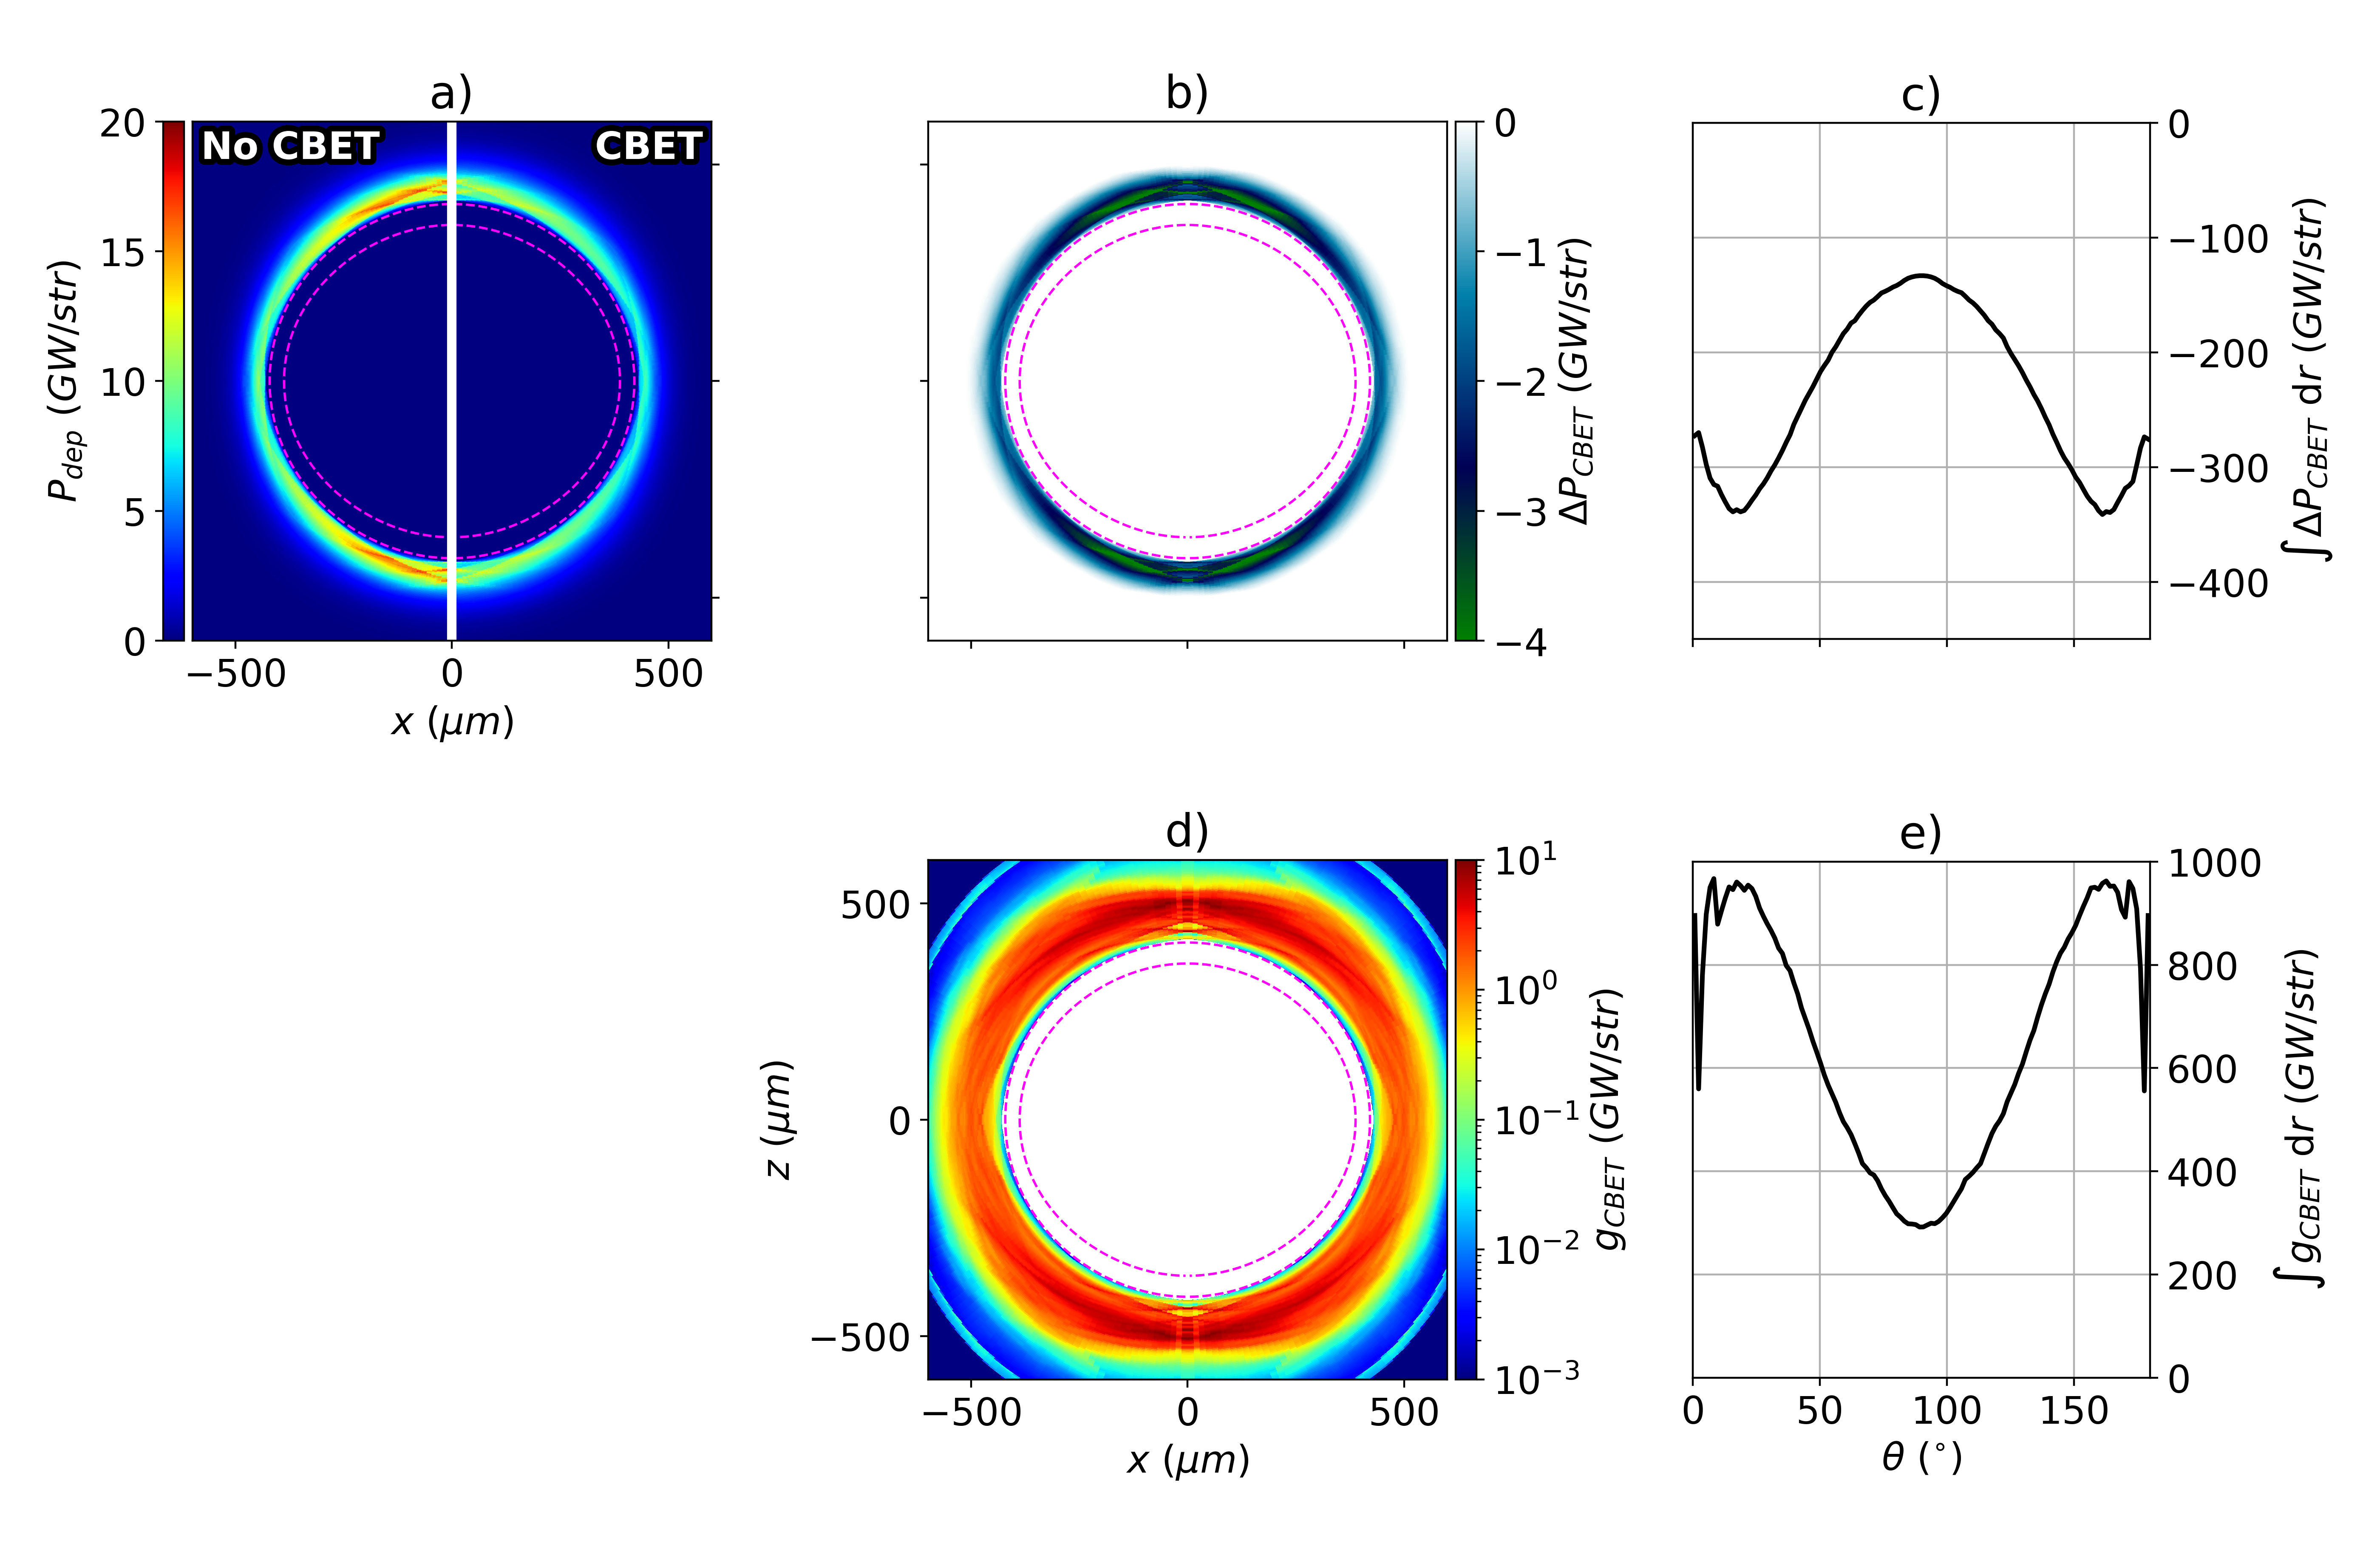
\includegraphics[width=\linewidth]{Results2/Images/magcbet_analysis.png}
    \centering
    \caption{Various \ac{CBET} diagnostics used in the analysis presented in this section.
    All plots are from the $B_{z0}=0\ \text{T}$, with-\ac{CBET} simulation at $t=0.30\ \text{ns}$.
    Panel a) plots the instantaneous deposition with (right-side) and without (left-side) the effect of \ac{CBET}.
    The `\ac{CBET}-deficit', $\Delta P_{\text{CBET}}$, which is the no-\ac{CBET} deposition, subtracted from the with-\ac{CBET} deposition, is plotted in panel b).
    Panel c) plots the radially integrated $\Delta P_{\text{CBET}}$, as a function of polar angle.
    The `\ac{CBET}-scattering', is plotted in panel d), and the radial integral is plotted in panel e).
    At this time, it is evident from panel e) that more \ac{CBET} occurred at the capsule poles, resulting in a \ac{CBET}-reduction of deposition near the poles, seen in panel c).
    The critical surface is shown in all 2-D panels by a dashed magenta line.}%
    \label{fig:Res2_magcbet_analysis}
\end{figure}

Firstly, key quantities used for the analysis of this section shall be introduced.
The key aim of this section was to discover if \ac{CBET} acted differently in the magnetised coronal hydrodynamic profiles, compared to the unmagnetised profiles.
Particular focus was dedicated to discovering if this affected the implosion shape, because this shape change would not be captured by a laser-\ac{MHD} model that did not have a full-\ac{CBET} capability, but rather reduced the incident laser energy to compensate for \ac{CBET}.
Two quantities were used to understand how \ac{CBET} redistributed the deposited power.
The first was the `\ac{CBET}-deficit', which is defined as the difference in deposited power computed by a \ac{CBET} and no-\ac{CBET} raytrace through the \textit{same} hydrodynamic profiles,
\begin{equation}
    \Delta P_{\text{dep}}(\vec{x},t) = P_{\text{dep}}^{\text{CBET}}(\vec{x},t) - P_{\text{dep}}^{\text{no-CBET}}(\vec{x},t),
\end{equation}
where $P_{\text{dep}}^{\text{CBET}}$ is the deposition from the calculation including \ac{CBET} and $P_{\text{dep}}^{\text{no-CBET}}(\vec{x},t)$ is without \ac{CBET}.
As was described in Sec.~\ref{SOLAS:pump_dep_iters}, a \ac{CBET} calculation in \textsc{Solas} always begins with a raytrace which does not include any \ac{CBET} effects (the field-reconstruction raytrace), so $P_{\text{dep}}^{\text{no-CBET}}(\vec{x},t)$ is the deposited power from this raytrace.
$P_{\text{dep}}^{\text{CBET}}(\vec{x},t)$ is the value after the pump depletion and energy conservation iterations, \textit{i.e.} after \ac{CBET} has been fully accounted for.

Fig.~\ref{fig:Res2_magcbet_analysis}.a plots the deposited power without (left-side) and with-\ac{CBET} (right-side), from the $B_{z0}=0\ \text{T}$, with-\ac{CBET} simulation at $t=0.30\ \text{ns}$.
The corresponding \ac{CBET} deficit, which is the difference between these plots, is shown in Fig.~\ref{fig:Res2_magcbet_analysis}.b.
Note that the value is almost all negative, because for direct-drive configurations, \ac{CBET} mainly acts to reduce the intensity of light near the critical surface where \ac{Inv-Brem} predominantly occurs, and therefore it reduces the deposited power.
There are small ($\sim$1\%) increases in deposition at radii outside the peak scattering surface, near Mach-1, but this increase is not be visible to the naked eye when the maximum colourbar scale is increased above zero.
It can be seen from the \ac{CBET} deficit, that at this time, \ac{CBET} decreased the absorption at the poles more than at the equator of the capsule.
This can be understood by considering the geometry of the pole heavy drive.
The beam geometry meant that the intensity was greater in the polar coronal plasma, where many beams overlapped each other.
Therefore, inbound laser sheets encountered stronger \ac{CBET} resonances, because more reflected sheets were present in this region, thus their energy was depleted more than at the waist.
The radial integral of the \ac{CBET} deficit is plotted in Fig.~\ref{fig:Res2_magcbet_analysis}.c.
This conveniently illustrates the previous point, that the reduction in absorption due to \ac{CBET} (at this time, of this simulation), was greater near the poles than the equator.
It is also worth noting, that if \ac{CBET} acted symmetrically to simply reduce the absorption rather than redistribute it, then Fig.~\ref{fig:Res2_magcbet_analysis}.c would be uniform in $\theta$.
This is the case for the `partial-\ac{CBET}' simulations, labelled by `$\sim$' under the \ac{CBET} column in Tab.~\ref{tab:Res2_magexpl_results}, where the magnitude of the power was reduced to account for \ac{CBET}, but the redistribution of power was not accounted for.

The second metric was the \ac{CBET} scattering, $G_{\text{CBET}}$, defined in Sec.~\ref{sec:SOLAS_89224}, but restated here for convenience,
\begin{equation}
    \label{sec:res1_cbet_scattering}
    g_{\text{CBET}}(\vec{x},t) = \sum_{i}^{\text{rays}} \left| \Delta P_{i,\text{CBET}}(\vec{x},t) \right|,
\end{equation}
where the time dependence has now been made explicit and $\Delta P_{i,\text{CBET}}$ is the power change of a ray due to \ac{CBET}.
This quantity shows where the majority of \ac{CBET} power change occurred, across the simulation domain, at a given time.
Fig.~\ref{fig:Res2_magcbet_analysis}.d plots $g_{\text{CBET}}$ on a log scale, from the same simulation and at the same time as Fig.~\ref{fig:Res2_magcbet_analysis}.a.
The radial integral of this plot is shown in Fig.~\ref{fig:Res2_magcbet_analysis}.e, as a function of angle.
It is evident by comparison of Fig.~\ref{fig:Res2_magcbet_analysis}.c and Fig.~\ref{fig:Res2_magcbet_analysis}.e, that the angles of maximal \ac{CBET} scattering align with the most significant deficits, and vice-versa.
It should be noted that there is some noise visible in both \ac{CBET} scattering plots near the poles.
This was presumed to be due to small cells and therefore poorer ray-per-cell statistics in this region.
This noise was, however, localised to a few polar-cells, and therefore not thought to have a significant impact on the overall dynamics.

%################################################################################
%################################################################################
\subsection{Spatial Change of CBET and Deposition from Magnetisation}%
\label{sec:Res2_mag_on_cbet_change}

\begin{figure}[t!]
    \includegraphics[width=\linewidth]{Results2/Images/Scattering_time_phi_diffCBET_CBtr.png}
    \centering
    \caption{The radially integrated \ac{CBET}-deficit and \ac{CBET}-scattering, plotted as a function of angle and time for the $B_{z0}=0$ and $50\ \text{T}$, with-\ac{CBET} simulations.
    Panel b) plots the \ac{CBET}-deficit from the 50 T (top-half) and 0 T (bottom-half) simulations.
    Lineouts in $\theta$ at $t=0.25$ (black), $0.50$ (dark-green) and $0.75\ \text{ns}$ (light-green) are plotted in panel a).
    The same results, but for \ac{CBET}-scattering are plotted in panels d) and c).
    It is evident from these plots that for both simulations, as time passed and the poles of the capsule fell in faster than the equator, the region where \ac{CBET} mostly occurred, shifted in angle around the capsule.
    Differences are visible in all plots between the $B_{z0}=0$ and $50\ \text{T}$ simulations, indicating that magnetisation affected \ac{CBET} indirectly, via the altered hydrodynamics.}%
    \label{fig:Res2_scattering}
\end{figure}

This section shall explore differences in the \ac{CBET}-deficit and \ac{CBET}-scattering, between magnetised and unmagnetised implosions.
As was illustrated in Fig.~\ref{sec:Res2_mag_on_CBET}, magnetisation significantly amplified coronal plasma asymmetries in direct-drive implosions.
Thus, an effect on the \ac{CBET} gain calculations was expected.
How changes to \ac{CBET} affect the hydrodynamics and stagnation shape of the target, is discussed in the subsequent Sec.~\ref{sec:Res2_stgnation_profiles}.

Fig.~\ref{fig:Res2_scattering}.b plots the \ac{CBET} deficit as a function of time ($x$ axis) and polar angle ($y$ axis) for the with-\ac{CBET}, $B_{z0}=50\ \text{T}$ (top-half) and $B_{z0}=0\ \text{T}$ (bottom-half) simulations respectively.
Note that the colour scale has a maximum of zero, and is most saturated at negative values, because the radially integrated \ac{CBET}-deficit was entirely negative.
Lineouts in $\theta$ at three times, $t=0.25$, $0.50$ and $0.75\ \text{ns}$ (times indicated by dashed lines on Fig.~\ref{fig:Res2_scattering}.b), are plotted in Fig.~\ref{fig:Res2_scattering}.a, where the $x$ axis of this plot share the colour scale from Fig.~\ref{fig:Res2_scattering}.b.
Broadly, both the top half and the bottom half of Fig.~\ref{fig:Res2_scattering}.b appear to be qualitatively similar, indicating that magnetisation of coronal profiles did not play a dominant role in altering \ac{CBET}.
The simulations featured a large \ac{CBET}-deficit of deposition near the poles between $t\sim0.2\rightarrow0.3\ \text{ns}$.
As the implosion progressed, the asymmetry of the deficit reduced, which is visible as the reducing saturation of the plot, with increasing time.
This was, however, also partially due to the lengthening of the plasma corona, which increased symmetry primarily through increasing deposition at larger radii.
Large radius deposition is less efficient at coupling to ablation, compared to if the energy were deposited close to critical, due to thermal conduction having to transport it further.
An improved metric, which appropriately weights deposition by distance from the critical surface, may further elucidate the role of \ac{CBET}.
Both plots show that the peak of the \ac{CBET}-deficit shifted to the equator as the simulations progressed.

The \ac{CBET}-scattering streak plot and lineouts in Fig.~\ref{fig:Res2_scattering}.d and~\ref{fig:Res2_scattering}.c respectively show similar behaviour.
Before $t\sim0.2\ \text{ns}$, the level of \ac{CBET}-scattering was low, primarily due to the low incident power, and therefore laser field strengths.
Maximal scattering occurred near the poles, at early times in both the magnetised and unmagnetised simulations, which then moved more to the equator later on.
The movement of the scattering and deficit to the equator was due to the asymmetric convergence of the target.
As can be seen from the time resolved $n_e$ profiles from the with-\ac{CBET} simulation in Fig.~\ref{fig:Res2_unmag_CBET_onoff}, the coronal plasma was relatively round up until $t\sim0.35\ \text{ns}$, but then began to implode more quickly along the $\pm\hat{\vec{z}}$ axis than the equator.
When this occurred, the trajectory of light changed asymmetrically, leading to a change of polar-angle where \ac{CBET} predominates.

Firstly, the expected change to the bangtime profiles from the similar, qualitative behaviour shall be described.
Bangtimes for these implosions were at $t\sim0.75\ \text{ns}$, so the late time behaviour shortly before and after this, was unimportant in dictating the bangtime shapes.
The most significant $\Delta P_{\text{CBET}}$ values occurred between $t\sim0.2\rightarrow0.3\ \text{ns}$ at the poles, for both the magnetised and magnetised simulation.
This \ac{CBET}-induced power redistribution, would have reduced the strength of the shock launch along the poles, compared to the equator.
Therefore, simulations with an equal magnitude of power deposition, but no spatial relocation of deposition (\textit{i.e.} the partial-\ac{CBET} simulations), were expected to exhibit a larger $\ell=2$ asymmetry, because \ac{CBET} appeared to reduce the asymmetry of the drive.

Now, the change to the \ac{CBET} deficit between the magnetised and unmagnetised simulations shall be explicitly compared.
If the altered coronal plasma profiles due to magnetisation had played a dominant role in changing \ac{CBET}, then the top and bottom plots would look markedly different.
The similar qualitative behaviour seems to suggest therefore that this is not the dominant role in dictating implosion symmetry.
However, minor differences are observable, for example the magnetised simulation exhibited more early-time \ac{CBET}-scattering and a slightly larger \ac{CBET}-deficit at the poles, which also lasted for a slightly longer period of time.
This suggests that the shock launch in the $B_{z0}=50\ \text{T}$ case would be slightly weaker than the $B_{z0}=0\ \text{T}$ case.
A significant reason for the relatively small changes, is that the pole-heavy drive obscures these, more subtle, changes to implosion dynamics.
Explicitly, an unmagnetised, symmetric drive beam-configuration should not display an $\ell=2$ asymmetry in either of the diagnostics, and should thus result in a mostly symmetric bangtime profile.
Changes to the shape, would therefore be much less obscured compared to these simulation which feature a global asymmetry, imposed by the 40-beam drive.

%################################################################################
%################################################################################
\subsection{Stagnation Profiles}%
\label{sec:Res2_stgnation_profiles}

\begin{figure}[t!]
    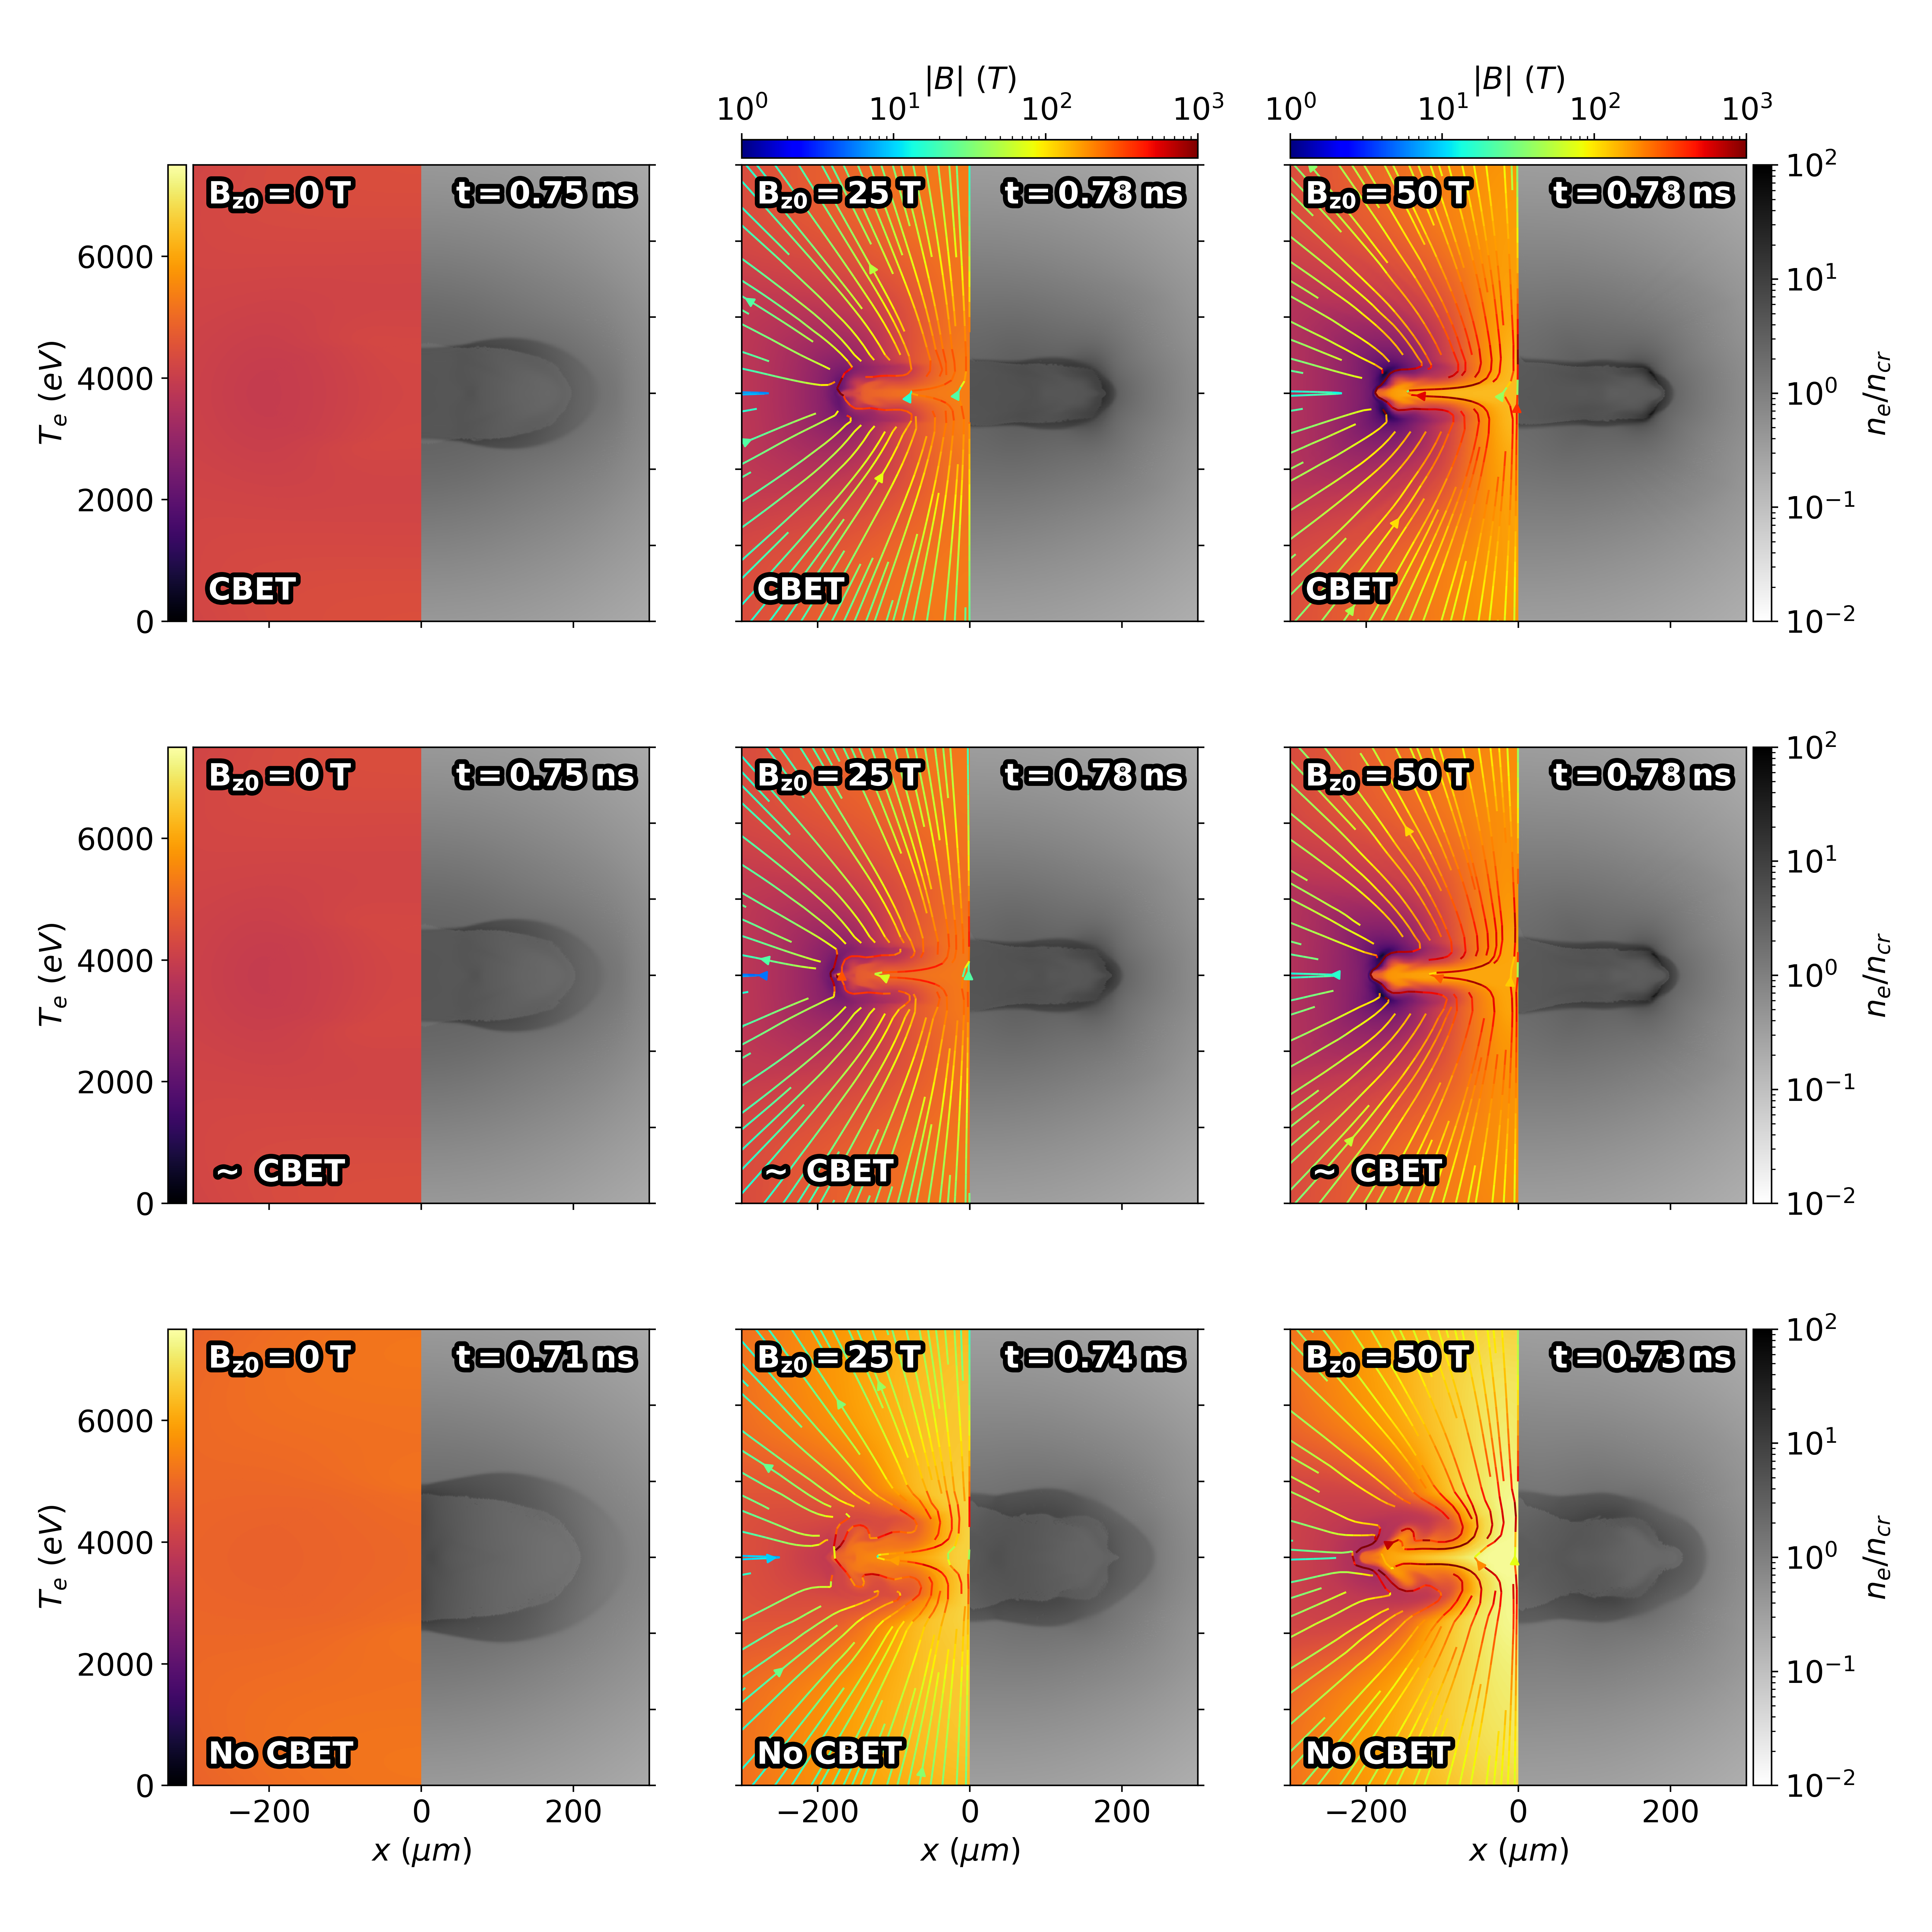
\includegraphics[width=\linewidth]{Results2/Images/allall_stagnation.png}
    \centering
    \caption{$n_e$, $T_e$ and $\vec{B}$ bangtime profiles for different initial magnetisation (columns) and \ac{CBET} treatments (rows).
    Panels a), b) and c) are from the full \ac{CBET} simulations, which show that magnetisation increased the oblateness of the stagnation profile.
    Panels d), e) and f) are from the simulations where only the \ac{CBET} effect on the magnitude, but not spatial location, of deposition was included.
    These simulations have identical coupled energy to the top row, and therefore have the same bangtimes.
    Panels g), h) and i) are from the no-\ac{CBET} simulations, which had earlier bangtimes and increased temperatures, due to the greater coupled energy.}%
    \label{fig:Res2_allall_stagnation}
\end{figure}

The bangtime $n_e$, $T_e$ and $\vec{B}$ profiles from the 2-D simulations with all magnetisations (columns) and all \ac{CBET} treatments (rows) are plotted in Fig.~\ref{fig:Res2_allall_stagnation}.
The top row of figures correspond to full \ac{CBET} treatment and the bottom row, no effect of \ac{CBET} is included.
As a reminder, to conduct the partial-\ac{CBET} simulations in the middle row (labelled `$\sim$\ac{CBET}' for shorthand), the deposited power as a function of time was loaded in from the (already completed) full-\ac{CBET} simulation with the same initial $B_{z0}$ value.
No-\ac{CBET} ray-traces were then conducted with incident power normalised to unity, and the deposition was multiplied by the absorbed power from the full-\ac{CBET} simulation at the same time.
Thus, full-\ac{CBET} and $\sim$\ac{CBET} simulations with equivalent $B_{z0}$ have identical power deposition as a function of time.
The only difference between them is that the full-\ac{CBET} simulations, on the top row, include redistribution of deposition around the corona.

Rows labelled run $2\rightarrow11$ in Tab.~\ref{tab:Res2_magexpl_results} provide the integrated metrics for each of these simulations.
The first thing to note about these results, is that all implosions were oblate, \textit{i.e.} the radius of peak density was significantly larger in the equatorial direction than polar.
Magnetisation also evidently flattened the implosion, regardless of \ac{CBET} treatment.
No-\ac{CBET} simulations (bottom row) were also significantly less oblate than the top two rows, which both included reduced absorption due to \ac{CBET}.
To remind the reader, it was due to the larger $|V_{r,\text{shock}} - V_{r,\text{shell}}|$ for the no-\ac{CBET} simulation, compared to when \ac{CBET} was included, as was described in~\ref{sec:Res2_expl2D}.
Thus, the collision between the rebounding shock and in-falling fuel material happened at larger radii, resulting in a rounder bangtime shape.

The stagnation field structure for the magnetised simulations exhibited field lines at $z\sim0\ \mu\text{m}$ which point along $\pm\hat{\vec{x}}$.
This was due to the oblate structure of the initial strong shock, which moved mainly along $\pm\hat{\vec{z}}$ for a wide array of $x$ values.
When the shocks from the two poles met at $z=0\ \mu\text{m}$, a thin layer was superheated to extreme temperatures of several $10 \text{keV}$.
This thin layer of highly conductive plasma, reoriented the un-shocked $+\hat{\vec{z}}$ field to point in the $\pm\hat{\vec{x}}$ directions.
The large compressed field strengths also increased the peak temperatures significantly, by insulating thermal losses.
Note however, that this increase was highly anisotropic and was localised to lower density regions of the hotspot, therefore did not directly translate to increased burn-averaged temperatures in Tab.~\ref{tab:Res2_magexpl_results}.
For simulations which exhibited larger hotspot temperatures, the higher pressures appeared to develop some form of magneto-\ac{RTI} at the equator of the capsule, most evidently visible in $T_e$ at $x,z\sim[-150,0]\ \mu\text{m}$, although the exact dynamics of this have not been studied in detail.

\begin{figure}[t!]
    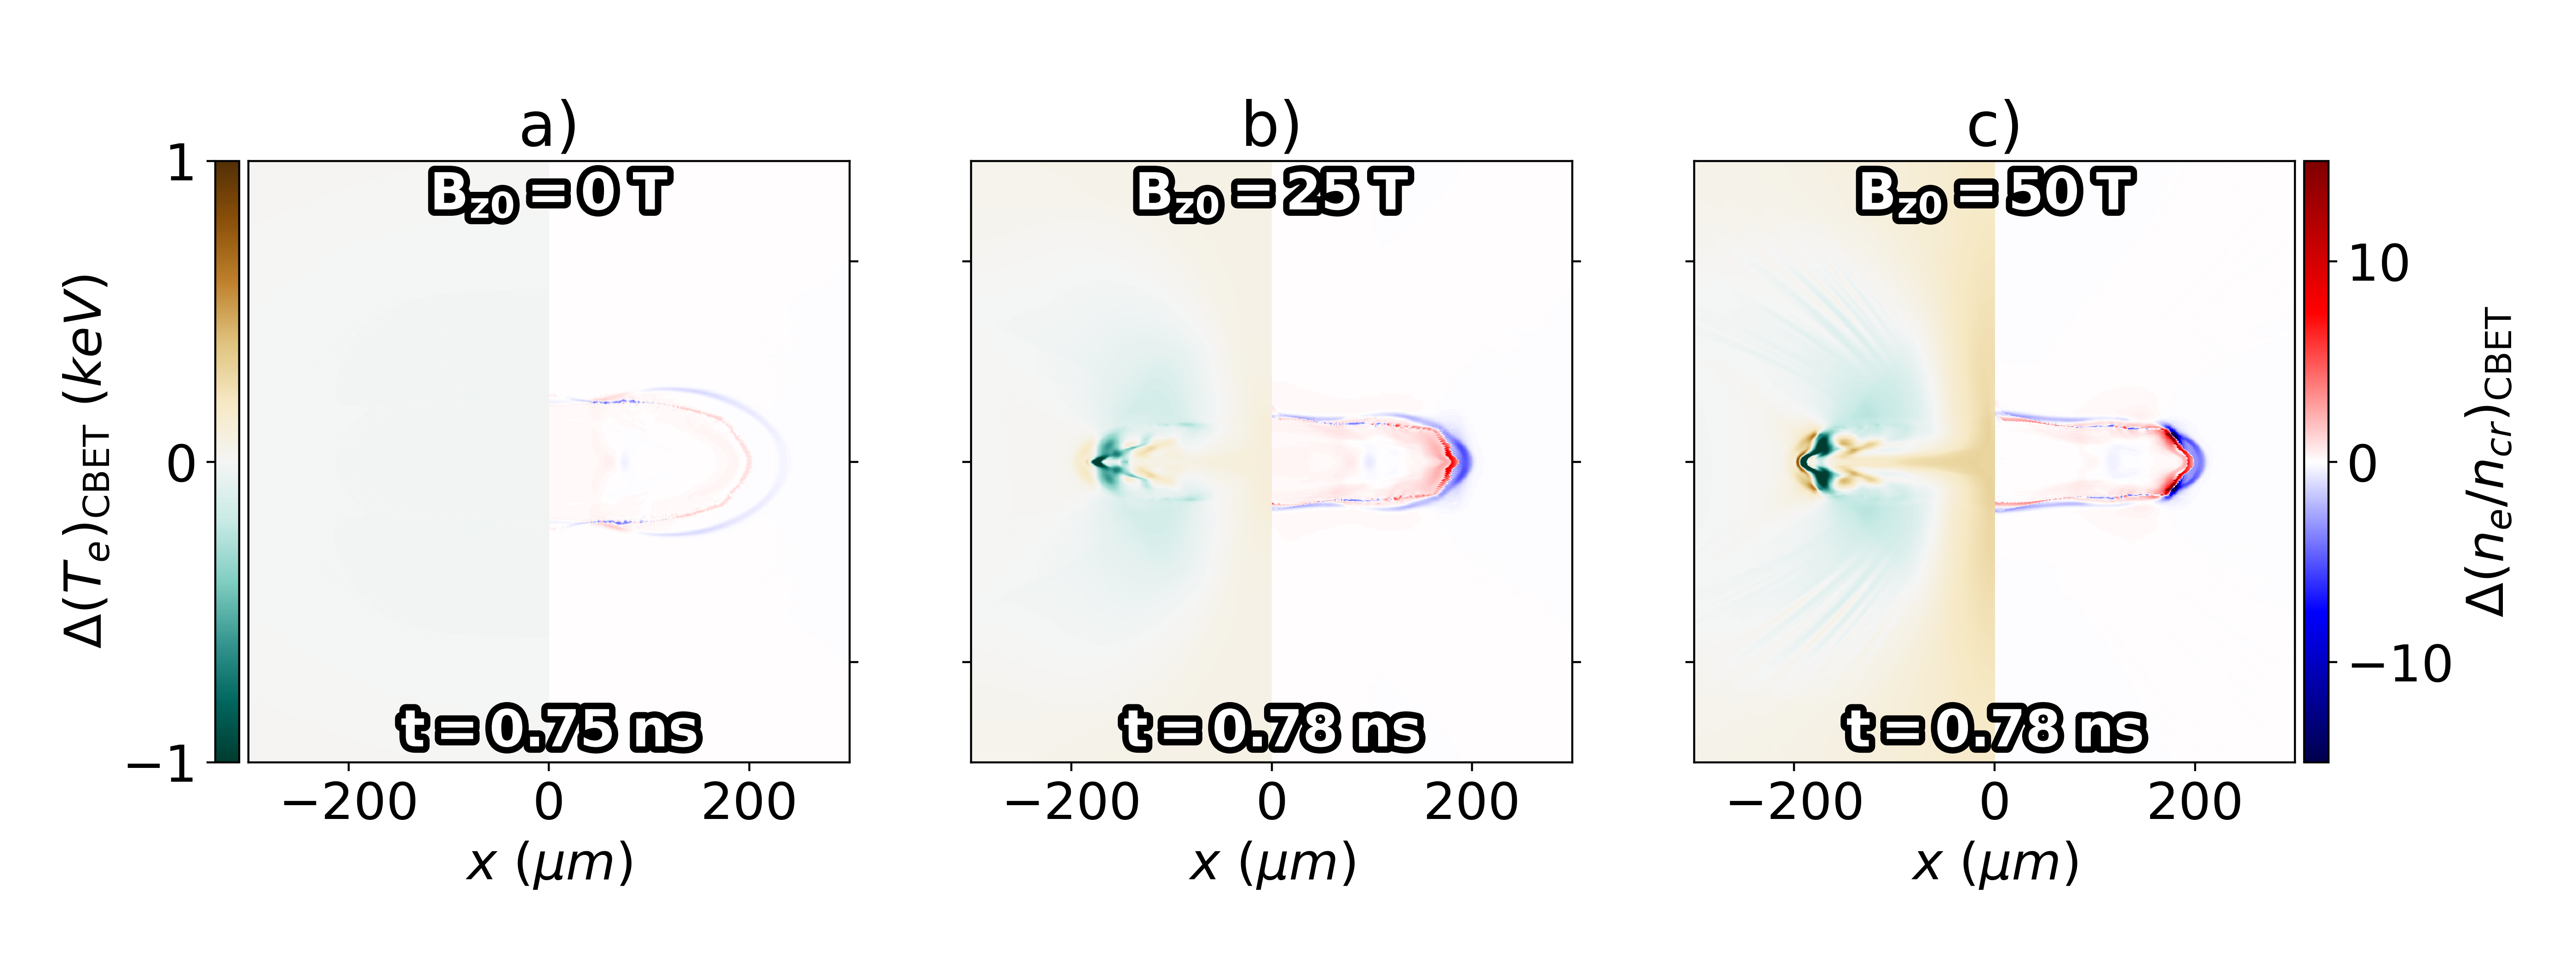
\includegraphics[width=\linewidth]{Results2/Images/CBETshape_stag_diff.png}
    \centering
    \caption{Difference in $n_e$ and $T_e$ bangtime profiles, between the full-\ac{CBET} and \ac{CBET}-magnitude a) $B_{z0}=0$, b) $B_{z0}=25$ and c) $B_{z0}=50\ \text{T}$ simulations.
    The difference in variable $v$, is defined as $\Delta v = v_{\text{full-CB}}-v_{\text{partial-CB}}$, so higher colour scale values represent regions with increased $v$ for the full-\ac{CBET} calculation.
    These results primarily show that \ac{CBET} slightly reduced the bangtime equatorial radius, and thus reduced the oblateness, compared to simulations where the spatial redistribution of power due to \ac{CBET} was neglected.}%
    \label{fig:Res2_CBETshape_diff}
\end{figure}

If \ac{CBET} was anisotropically affected by magnetisation, this would result in spatial differences in deposition location, between the full \ac{CBET} (top row) and partial-\ac{CBET} simulations (middle row), and therefore the bangtime profiles would be different.
Additionally, higher initial magnetisation increased the coronal plasma anisotropy.
Therefore, the difference between the top two rows would have changed as $B_{z0}$ increased, \textit{i.e.} from column to column.
Evidently, the top rows appear very similar to each other, which illustrates that anisotropic changes to \ac{CBET} from magnetised hydrodynamic profiles was a small effect compared to both the polar nature of the drive and the anisotropic drive due to magnetised transport.
Small changes are present however, which is far more clearly displayed in Fig.~\ref{fig:Res2_CBETshape_diff}.
This figure plots the difference in $n_e$ and $T_e$ between the full-\ac{CBET} (top row of~\ref{fig:Res2_allall_stagnation}) and partial-\ac{CBET} (middle row of~\ref{fig:Res2_allall_stagnation}) bangtime profiles.
As can be seen, differences became more significant at larger magnetisations, demonstrating that anisotropic changes of \ac{CBET} scattering do impact upon the hydrodynamics.
The main difference can be seen at the equator of the $n_e$ profile, of both magnetised simulations, where the full-\ac{CBET} maximum density occurs at a lower $x$ value.
Thus, \ac{CBET} redistribution of deposition in magnetised coronal profiles marginally reduced the oblateness of the bangtime density.
This aligns with the expected behaviour, described at the end of Sec.~\ref{sec:Res2_mag_on_cbet_change}.
Restating here, the early, localised \ac{CBET}-deficit reduced the strength of the polar shock launch compared to the equatorial shock.
This improved the symmetry of the shock and therefore the stagnation state.
It was also observed that this effect seemed to become marginally more significant in magnetised coronal profiles.
By comparing Fig.~\ref{fig:Res2_CBETshape_diff}.a with Fig.~\ref{fig:Res2_CBETshape_diff}.b and~\ref{fig:Res2_CBETshape_diff}.c, the differences are slightly more significant, which supports this analysis.

\begin{figure}[t!]
    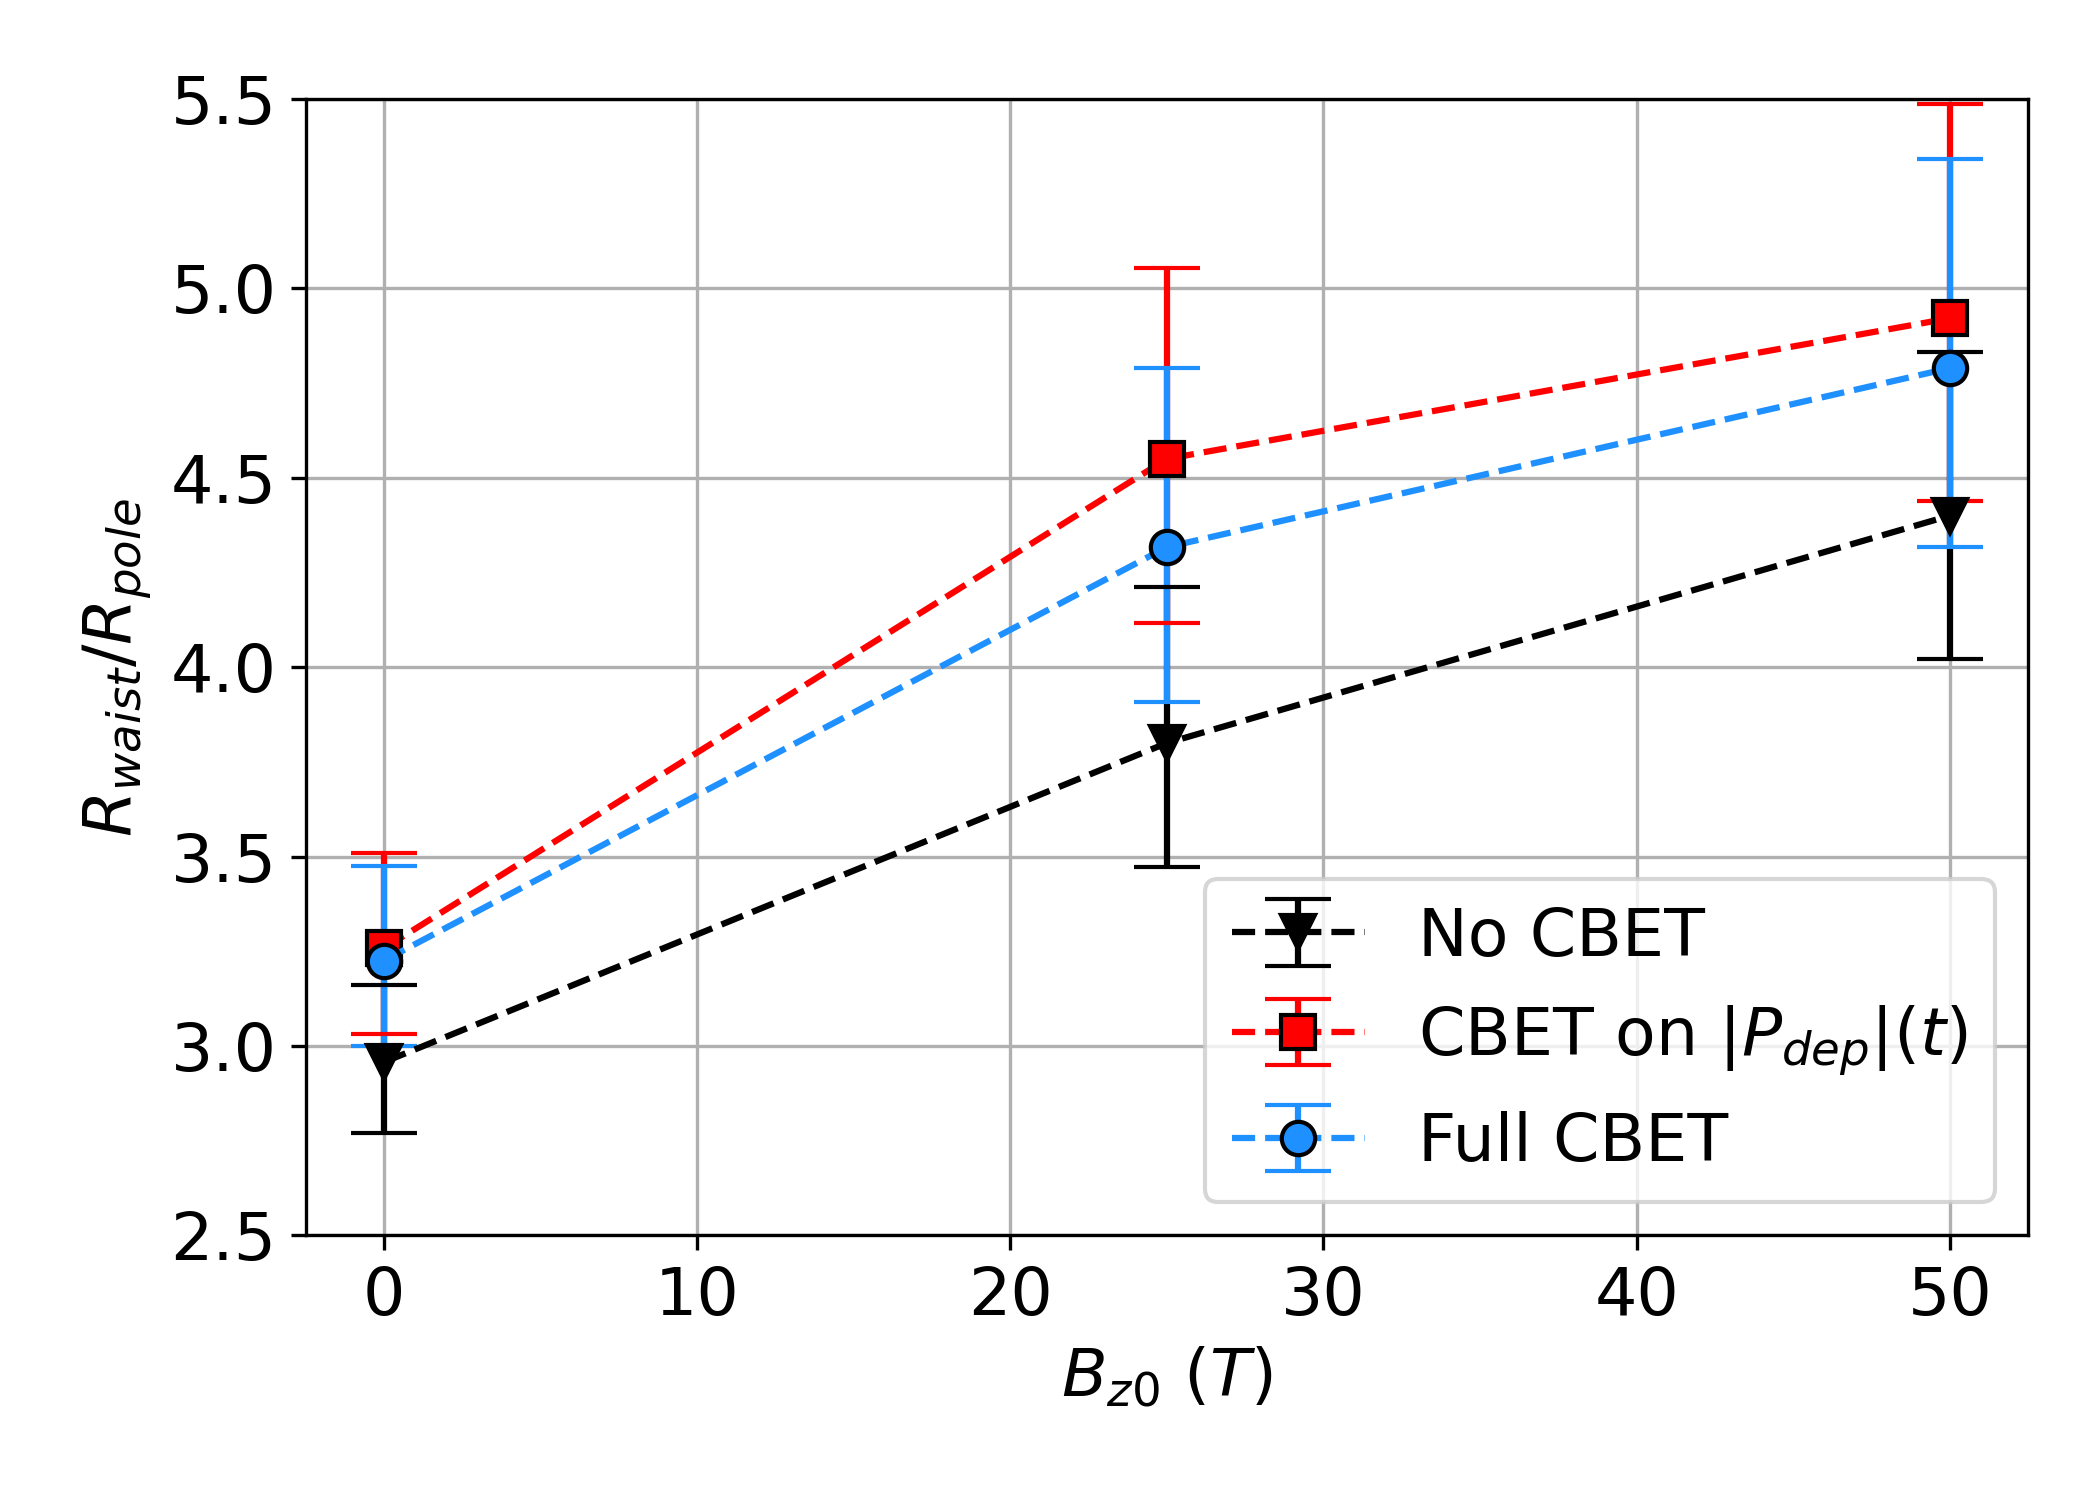
\includegraphics[width=0.6\linewidth]{Results2/Images/R2R0_errors.png}
    \centering
    \caption{The oblateness of bangtime density profiles for different magnetisation and \ac{CBET} effects.
    All values and errors were obtained by fitting an ellipse (with axes orientated along $\hat{\vec{x}}$ and $\hat{\vec{z}}$), to the radius of maximum density.
    No-\ac{CBET} simulations were consistently more round, because the initial shock was stronger, and therefore travelled ahead of the pusher material more quickly than the \ac{CBET} equivalent.
    Thus, after rebounding off the axis, it met the infalling mass and produced thermonuclear conditions at a larger radius.
    As was seen in Fig.~\ref{fig:Res2_CBETshape_diff}, throughout the entire implosion, when the effect of \ac{CBET} on spatial location of deposition was included, it acted to slightly move energy from the pole to the waist and thus marginally reduced the oblateness of the stagnation state.}%
    \label{fig:Res2_R2R0_errors}
\end{figure}

The oblateness parameters from Tab.~\ref{tab:Res2_magexpl_results} are plotted for these implosions as a function of initial field strength for different \ac{CBET} treatments.
These values were obtained by fitting an ellipse to the contour of maximum density at bangtime.
The fitting procedure returned asymmetric error bars, which are also plotted.
As was observed by examining the profiles in Fig.~\ref{fig:Res2_allall_stagnation} directly, the no-\ac{CBET} results are all significantly rounder, compared to simulations for which the effect of \ac{CBET} on deposition magnitude is included.
This was due to the faster shock launched with greater early time deposition.
The partial-\ac{CBET} simulations, which do not include redistribution of deposition are all marginally more oblate than the full-\ac{CBET} simulations, with the caveat this cannot be stated conclusively, because of the error bar magnitudes.
Simply stated, \ac{CBET} acts to slightly reduce the oblateness of the stagnation state by effectively redistributing a small quantity of power from the poles of the capsule to the equator.
There is no evidence from this plot, however, that increasing magnetisation, anisotropically alters \ac{CBET} sufficiently to leave an experimental signature.
If, for example, the difference between the full- and partial-\ac{CBET} curves had diverged (or converged) with increasing magnetisation, this would have suggested that the increasingly anisotropic hydrodynamic profiles from magnetisation, significantly impacted upon the \ac{CBET} scattering.

In retrospect, however, it was noted that the configuration used for these simulations likely minimised any observable effect in several ways.
Firstly, as was discussed at the end of Sec.~\ref{sec:Res2_mag_on_cbet_change}, the polar beam geometry obscured the less significant \ac{CBET} anisotropy from magnetisation.
Secondly, the shock driven nature of the exploding-pusher configuration, could have minimised experimentally observable signatures.
The shape of the stagnation state was predominantly dictated by the shock launch geometry from the shell explosion, which was mostly sensitive to the early laser-energy deposition.
A more conventional, hotspot ignition target would have maintained a dense shell throughout the implosion, which would have developed density modulations due to \ac{CBET}-induced deposition asymmetries, as was seen in the previous chapter, for example in Fig.~\ref{fig:Res1_stagnation_plots}.
Experimentally, a mode $\ell=2$ is long wavelength enough to be inferred from neutron diagnostics, and would thus leave an experimentally observable signature in the neutron spectrum~\cite{woo_impact_2018,casey_three_2021}.
Finally, higher $Z$ ablator materials such as $\text{SiO}_2$, exhibit higher coronal plasma temperatures than CH shells, due to increased \ac{Inv-Brem} efficiency.
\ac{CBET} becomes less significant for direct-drive, as the coronal temperatures increase~\cite{colaitis_exploration_2023}, therefore an experimental setup with a CH outer material, may have lead to more \ac{CBET} scattering overall, and therefore a more easily observable change to hydrodynamic profiles from magnetisation.

%###############################################################################################################################
%###############################################################################################################################
%###############################################################################################################################
\section{Conclusions}%
\label{sec:Res2_conclusions}

%################################################################################
%################################################################################
\subsection{Summary of Work}%
\label{sec:Res2_summary}

This chapter has described simulations of directly-driven, magnetised exploding-pusher implosions.
For the first time, an in-line model for \ac{CBET} was included in a magnetised direct-drive implosion simulation, in order to study how asymmetry in coronal plasma profiles from magnetisation, may affect the action of \ac{CBET}.
1-D simulations of the exploding-pusher configuration without magnetisation demonstrated that \ac{CBET} was dynamically significant to the implosion, reducing the coupled laser energy to the target by $10\rightarrow15\%$.
The main effect of this reduced absorption was to slow the speed of the strong shock, which led to bangtime occurring at greater target convergence after the rebounding shock compressed against the in-falling material.
When extended to 2-D, the simulations demonstrated that the polar nature of the drive was highly significant to the symmetry of the implosion, leading to a bangtime density profile with an aspect ratio $R_{\text{eq.}}/R_{\text{pole}}\sim 3$.
The slowing of the shock due to the \ac{CBET} reduction of absorption, led to bangtime occurring at a larger radius, and thus a less oblate profile was obtained, because the shock travelled mainly along the $\pm\hat{\vec{z}}$-axis.
Simulations which included the reduced absorption due to \ac{CBET}, but not spatial redistribution of energy, showed that \ac{CBET} power redistribution marginally reduced the oblateness of the implosion, consistent with how it acts to reduce $\ell=1$ asymmetries~\cite{anderson_effect_2020}.

Simulations were also conducted which included an initial magnetic field along the $+\hat{\vec{z}}$-axis.
The key physical processes which were dynamically significant to the implosion dynamics were identified by conducting additional simulations which turned off the effect of each process in turn.
Anisotropic thermal conduction was shown to be highly significant.
It acted to insulate the deposited energy at the poles of the equator, preventing thermal equilibration in the polar direction and thus led to an increased asymmetry of the drive.
The generally high temperatures of the target led to large $R_m$ and Plasma $\beta$ values, therefore the Lorentz force and resistive diffusion had minimal impact on the implosion.
Nernst advection of the magnetic field effectively reoriented the coronal field structure at the low-Hall parameter, equator of the target.
This field reorientation altered the anisotropic thermal conduction, leading to a `bump' in the density at the target waist.
Although this equatorial-bump had minimal impact on integrated neutron diagnostics, because it was well removed from the polar-regions, which produced the most thermonuclear reactions, it may significantly impact yields for symmetrically driven targets.

The impact of the magnetised coronal plasma profiles on \ac{CBET} scattering of the laser energy was also studied.
By examining how \ac{CBET} reduced absorption instantaneously through both the magnetised and unmagnetised coronas, the dominant effect of \ac{CBET} was observed to be an early reduction of deposition at the capsule poles, regardless of seed field strength.
This led to a marginally more symmetric drive, reducing the oblateness of the bangtime profiles.
Increasing the level of the initial seed magnetic field appeared to slightly exaggerate this early, polar reduction of deposition, although the effect was minimal and did not significantly impact upon the hydrodynamics.
Therefore, increased anisotropy of the coronal field profiles was not observed to significantly alter \ac{CBET} scattering for these pole-heavy drive, exploding-pusher targets.

%################################################################################
%################################################################################
\subsection{Future Work}%
\label{sec:Res2_future}

Future alterations to the simulation configuration shall now be suggested, which may lead to a more obvious impact of magnetisation on \ac{CBET}.
The simulations that were conducted for this work all used a 40-beam \textsc{Omega} configuration, where the 20 equatorial beams were removed from the drive, due to the presence of a magnetic field coil in experiments.
Simulations demonstrated that this was the dominant effect, which dictated the symmetry of the bangtime state.
Magnetisation of thermal conduction also played a significant role, increasing the oblateness of the drive.
The polar drive largely obscured the much more subtle changes to \ac{CBET} from the altered hydrodynamic profiles, shown by comparing the top and bottom halves of panels in Fig.~\ref{fig:Res2_scattering}.
A configuration with a more symmetric, 60-beam drive, would not have an underlying $\ell=2$ anisotropy without magnetisation, which may make the changes to \ac{CBET} in magnetised profiles more pronounced.

Secondly, alterations to the target could be made which may lead to both increased diagnostic signatures of an anisotropic drive and a larger impact of \ac{CBET} overall.
Firstly, simulations of a more conventional, central hotspot ignition target could be conducted, which maintain a dense shell throughout the implosion.
Asymmetry of the deposition seeds density perturbations in the shell throughout the duration of the implosion.
This is in contrast to the exploding-pusher targets presented here, where the bangtime symmetry is predominantly dictated by the shape of the early, shock launch.
Additionally, using an ablator material with a lower ionisation state would lower the coronal plasma temperatures significantly and thus enhance the levels of \ac{CBET}~\cite{colaitis_exploration_2023}.
More subtle changes to \ac{CBET} scattering from magnetisation may thus have a larger impact on the implosion, due to more \ac{CBET} occurring overall.
